% !TeX root = tese.tex
%%% Exemplo de utilização da classe ITA
%%%
%%%   por        Fábio Fagundes Silveira   -  ffs [at] ita [dot] br
%%%              Benedito C. O. Maciel     -  bcmaciel [at] ita [dot] br
%%%              Giovani Volnei Meinertz   -  giovani [at] ita [dot] br
%%%    	         Hudson Alberto Bode       -  bode [at] ita [dot]br
%%%    	         P. I. Braga de Queiroz    -  pi [at] ita [dot] br
%%%    	         Jorge A. B. Gripp         -  gripp [at] ita [dot] br
%%%    	         Juliano Monte-Mor         -  jamontemor [at] yahoo [dot] com [dot] br
%%%    	         Tarcisio A. B. Gripp      -  tarcisio.gripp [at] gmail [dot] com
%%%
%%%   Versão para overleaf:
%%%   por        Alejandro A. Rios Cruz    - aarc.88@gmail.com
%%%              Saulo Gómez               - sagomezs@unal.edu.co
%%%              Ocimar Santos             - ocimar.acad@gmail.com
%%%
%%%   Template disponibilizado em:
%%%              Overleaf: https://pt.overleaf.com/latex/templates/thesis-template-aeronautics-institute-of-technology-ita/yhfrqqydpygk
%%%
%%%   Contribuia você também!
%%%              GitHub:   https://github.com/AlejandroRios/Template_Thesis_ITA
%%%
%%%  IMPORTANTE: O texto contido neste exemplo nao significa absolutamente nada.  :-)
%%%              O intuito aqui eh demonstrar os comandos criados na classe e suas
%%%              respectivas utilizacoes.
%%%
%%%  Tese.tex  2016-08-25
%%%  $HeadURL: http://www.apgita.org.br/apgita/teses-e-latex.php $
%%%
%%% ITALUS
%%% Instituto Tecnológico de Aeronáutica --- ITA, Sao Jose dos Campos, Brasil
%%%                   http://groups.yahoo.com/group/italus/
%%% Discussion list: italus {at} yahoogroups.com
%%%
%++++++++++++++++++++++++++++++++++++++++++++++++++++++++++++++++++++++++++++++
% Para alterar o TIPO DE DOCUMENTO, preencher a linha abaixo \documentclass[?]{?}
  % \documentclass[tg]{ita}			= Trabalho de Graduacao
%   \documentclass[tgfem]{ita}	= Para Engenheiras
%   								msc     		= Dissertacao de Mestrado
%   								mscfem   		= Para Mestras
%   								dsc      		= Tese de Doutorado
%   								dscfem   		= Para Doutoras
%   								quali    		= Exame de Qualificacao
%   								qualifem 		= Exame de Qualificacao para Doutoras
% Para 'Draft Version'/'Versao Preliminar' com data no rodape, adicionar 'dv':
%   \documentclass[dsc, dv]{ita}
% Para trabalhos em Inglês, adicionar 'eng':
%   \documentclass[dsc, eng]{ita}
%		\documentclass[dsc, eng, dv]{ita}
%++++++++++++++++++++++++++++++++++++++++++++++++++++++++++++++++++++++++++++++
\documentclass[tg, eng, dv]{ita}    % ITA.cls based on standard book.cls
% Quando alterar a classe, por exemplo de [msc] para [msc, eng]) rode mais uma vez o botão BUILD OUTPUT caso haja erro
\usepackage{ae}
\usepackage{graphicx}
\usepackage{epsfig}
\usepackage{amsmath}
\usepackage{amssymb}
\usepackage{subfig}
\usepackage{multirow}
\usepackage{float}
\usepackage{amsthm}
\usepackage{url}         % formats URL addresses properly
\usepackage{appendix}    % allows appendix section to be included
\usepackage{lscape}      % allows a page to be rendered in landscape mode
\usepackage{multicol}    % allows text in multi columns
\usepackage{cancel}      % needed to show canceled terms in equations
\usepackage{lettrine}
\usepackage{float}
\usepackage{placeins}
% \usepackage{natbib} % for references within the sentence
% \usepackage[backend=biber,style=authoryear]{biblatex}
% \addbibresource{References/references.bib} % troque pelo nome do seu arquivo .bib
%HHHHHHHHHHHHHHHHHHHHHHHHHHHHHHHHHHHHHHHHHHHHHHHHHHHHHHHHHHHHHHHHHHHHHHHHHHHHHHHHHHHHHHHHHHHHHHHHHHHHHHHHHHHH
%\usepackage{subfigure}
%\usepackage{subfigmat}
%PACOTEFIGURAS_SE _ERRADO_ESXCLUIR_ACIMA
\usepackage{multirow}  % para unir células na vertical
\usepackage{booktabs} % para toprule, midrule e bottomrule
\usepackage{array} % para definir colunas de tabelas com largura fixa

% Custom commands
\newcommand{\degree}{^{\circ}} % Shortcut for degree symbol in math mode
%PACOTETABELAS_SE _ERRADO_ESXCLUIR_ACIMA
%HHHHHHHHHHHHHHHHHHHHHHHHHHHHHHHHHHHHHHHHHHHHHHHHHHHHHHHHHHHHHHHHHHHHHHHHHHHHHHHHHHHHHHHHHHHHHHHHHHHHHHHHHHHH

%++++++++++++++++++++++++++++++++++++++++++++++++++++++++++++++++++++++++++++++
% Espaçamento padrão de todo o documento
%++++++++++++++++++++++++++++++++++++++++++++++++++++++++++++++++++++++++++++++
\onehalfspacing

%singlespacing Para um espaçamento simples
%onehalfspacing Para um espaçamento de 1,5
%doublespacing Para um espaçamento duplo

%++++++++++++++++++++++++++++++++++++++++++++++++++++++++++++++++++++++++++++++
% Identificacoes (se o trabalho for em inglês, insira os dados em inglês)
% Para entradas abreviadas de Professora (Profa.) em português escreva: Prof$^\textnormal{a}$.
%++++++++++++++++++++++++++++++++++++++++++++++++++++++++++++++++++++++++++++++
\course{Civil-Aeronautics Engineering}  % Programa de PG ou Curso de Graduação
%\area{Aircraft Design} % Área de concentração na PG (Não utilizado no caso de TG)

% Autor do trabalho: Nome Sobrenome
\authorgender{masc}                     %sexo: masc ou fem
\author{Felipe Mello}{dos Reis}
\itaauthoraddress{Rua H8A, Ap. 113}{12.228-460}{São José dos Campos--SP}

% Titulo da Tese/Dissertação
\title{Development of one-part alkali-activated cement with low-calcium solid precursors and alternative alkaline sources.}

% Orientador
\advisorgender{masc}                    % masc ou fem
\advisor{Prof.~Dr.}{João Cláudio Bassan de Moraes}{ITA}

% Coorientador (Caso não haja coorientador, colocar ambas as variáveis \coadvisorgender e \coadvisor comentadas, com um % na frente)
\coadvisorgender{fem}									% masc ou fem
% \coadvisor{Prof$^\textnormal{a}$.~Dr$^\textnormal{a}$.}{Doralice Serra}{OVNI}
\coadvisor{}{Pamela Rodrigues Passos Severino}{ITA}

% Pró-reitor da Pós-graduação
\bossgender{masc}												% masc ou fem
\boss{Prof.~Dr.}{Celso Massaki Hirata}

%Coordenador do curso no caso de TG
\bosscoursegender{fem}									% masc ou fem
\bosscourse{Prof$^\textnormal{a}$.~Dr$^\textnormal{a}$.}{Cláudia Azevedo Pereira}

% Palavras-Chaves informadas pela Biblioteca -> utilizada na CIP
\kwcip{Alkali activated material}
\kwcip{Geopolymer}
\kwcip{One-part}

% membros da banca examinadora

\examiner{Prof. Dr.}{Alan Turing}{Presidente}{ITA}
\examiner{Prof. Dr.}{Linus Torwald}{}{UXXX}
\examiner{Prof. Dr.}{Richard Stallman}{}{UYYY}
\examiner{Prof. Dr.}{Donald Duck}{}{DYSNEY}
\examiner{Prof. Dr.}{Mickey Mouse}{}{DISNEY}

% Data da defesa (mês em maiúsculo, se trabalho em inglês, e minúsculo se trabalho em português)
\date{26}{maio}{2025}

% Número CDU - (somente para TG)
\cdu{???.??}

% Glossario
\makeglossary
\frontmatter

\begin{document}
% Cover Page and Title Page for the TG case
\maketitle

% Dedication: Don't forget this section ... :-)
\begin{itadedication}
To the friends from Undergraduate and Graduate studies at ITA for motivating both the creation of this template by Fábio Fagundes Silveira and encouraging me and others to update and improve this excellent work.
\end{itadedication}

% Acknowledgments
\begin{itathanks}
First of all, I would like to thank Dr. Donald E. Knuth for developing \TeX.

To Dr. Leslie Lamport, for creating \LaTeX, greatly facilitating the use of \TeX, and thus, saving me from having to use Word.

To Prof. Dr. My Advisor, for the guidance and trust placed in the completion of this work.

To Dr. Nelson D'Ávilla, for lending his name to this important road in the city of São José dos Campos.

Oh, I almost forgot... I also thank \TeX, once again, for not having macro viruses :-)

\end{itathanks}

% Epigraph
\thispagestyle{empty}
\ifhyperref\pdfbookmark[0]{\nameepigraphe}{epigraph}\fi
\begin{flushright}
\begin{spacing}{1}
\mbox{}\vfill
{\sffamily\itshape
``If I have seen farther than others,\\
it is because I stood on the shoulders of giants.''\\}
--- \textsc{Sir~Isaac Newton}

\end{spacing}
\end{flushright}

% Resumo (in Portuguese)
\begin{abstract}
\noindent
Na busca por alternativas mais sustentáveis ao cimento Portland, os cimentos ativados alcalinamente têm sido amplamente estudados.
Inicialmente, a maioria dos processos de mistura ocorre em duas etapas, que sacrificam a eficiência produtiva em função das melhores proriedades mecânicas.
Com o objetivo  aumentar a escalabilidade do processo, o desenvolvimento de sistemas monocomponentes trouxe uma tecnologia mais acessível e prática para a indústria.
Ainda assim, os estudos atuais se concentram em precursores ricos em
cálcio, enquanto o uso de fontes alcalinas tradicionais apresenta desafios relacionados à segurança e ao custo.
Este trabalho propõe o desenvolvimento de um cimento ativado alcalinamente monocomponente utilizando precursores sólidos de baixo teor de cálcio, como sílica ativa e metacaulim, e fontes alcalinas mais seguras e acessíveis, como carbonato de potássio e hidróxido de cálcio, garantindo resistência mecânica adequada e maior viabilidade para aplicação na construção civil.
\end{abstract}

% Abstract (in English)
\begin{englishabstract}
\noindent
In the search for more sustainable alternatives to Portland cement, alkali-activated cements have been extensively studied. However, most mixing processes occur in two separate steps, limiting their feasibility and constructive efficiency. A significant advancement in this field is the development of one-part (just-add-water) systems, which simplify production and make the technology more accessible and practical. Nonetheless, current studies mainly focus on calcium-rich precursors, while the use of conventional alkaline activators raises concerns related to safety and cost. This work proposes the development of a one-part alkali-activated cement using low-calcium solid precursors, such as silica fume and metakaolin, along with safer and more affordable alkaline sources, such as potassium carbonate and calcium hydroxide. The goal is to ensure adequate mechanical performance while enhancing the viability of these materials for application in the construction industry.
\end{englishabstract}

% List of Figures
\listoffigures %optional

% List of Tables
\listoftables %optional

% List of Abbreviations
\listofabbreviations
\begin{longtable}{ll}
$CO_2$ & carbon dioxide \\
GHG & greenhouse gases \\
SCM & supplementary cementitious materials \\
AAM & alkali-activated materials \\
$ SiO_2$ & silica \\
$ Al_2O_3$ & alumina \\
N-A-S-H & sodium aluminate silicate hydrate \\
C-A-S-H & calcium aluminate silicate hydrate  \\
$K_2CO_3$ & potassium carbonate \\
$Ca(OH)_2$ & calcium hydroxide \\
MK & metakaolin \\
SF & silica fume \\
IPT & Institute for Technological Research \\
ITA & Aeronautics Institute of Technology \\
EDS & Energy dispersive X-ray spectroscopy \\
XRD & X-ray diffraction \\
$OH^-$ & hydroxyl \\
FTIR & Fourier transform infrared spectroscopy \\
ABNT & Brazilian Association of Technical Standards \\
NBR & Brazilian Standard \\
ASTM & American Society for Testing and Materials \\
OPC & Ordinary Portland Cement \\
GGBFS & Ground Granulated Blast Furnace Slag \\
MSWIA & Municipal Solid Waste Incineration Ash \\
NaOH & sodium hydroxide \\
Na$_2$SiO$_3$ & sodium silicate \\
KOH & potassium hydroxide \\
Na$_2$CO$_3$ & sodium carbonate \\
PSD & particle size distribution \\
LOI & loss on ignition \\
MIP & mercury intrusion porosimetry \\
IPT & Instituto de Pesquisas Tecnológicas \\
\end{longtable} %optional

% List of Symbols
\listofsymbols
\begin{longtable}{ll}
$a$ & Distance\\
$\textbf{a}$ & Distance vector\\
$\textbf{e}_{j}$ & Unit vector of dimension $n$ with the $j$-th component equal to $1$ \\
$\textbf{K}$ & Stiffness matrix\\
$m_1$ & Termite mass\\
$\delta_{k-k_f}$ & Kronecker delta at instant $k_f$\\
\end{longtable}

 %optional

% Table of Contents
\tableofcontents


\mainmatter
% Os capitulos comecam aqui

\chapter{Introduction}
Cement is one of the main materials in civil construction, being used from the construction of houses and buildings to bridges and highways.
In developing countries such as Brazil, cement is widely used due to its low complexity and cost, which allows its use on a large scale in any location.
The exponential increase in cement production, 10 times greater than the world population growth \cite{united1995world}, has been accompanied by a significant share of greenhouse gas (GHG) emissions, due to the calcination process of limestone that transforms calcium carbonate into calcium oxide and carbon dioxide in high-temperature furnaces.
The production of Portland cement generates on average 842 kg of $CO_2/t$ of clinker produced \cite{andrew2018global}, representing 5\% of anthropogenic GHG emissions \cite{IEA_WBCSD_2009}.

In this context, there is a need to develop new cementitious materials that present three main properties: low GHG emissions, low cost, and high strength/durability \cite{scrivener2018eco}.

Alkaline-activated materials (AAM) - solid precursors rich in silica ($SiO_2$) and alumina ($Al_2O_3$), capable of forming binding gels composed of sodium-alumino-silicate hydrate (N-A-S-H) and calcium-alumino-silicate hydrate (C-A-S-H) - have gained prominence due to their potential to partially or totally replace Portland cement, significantly reducing the GHG emissions associated with conventional cement production.

There are two ways in which AAM can be produced: by mixing the solid precursor with a liquid alkaline activator, or with a solid alkaline source and water.
Two-part systems have been widely employed in the initial development of this market due to their high mechanical performance, durability, and chemical resistance.
However, one-part systems are a more scalable technology due to the lower risk of handling and storing of solid activators \cite{provis2018alkali}.

Calcium-rich solid precursors are more used for several factors, such as the rapid strength gain \cite{provis2014geopolymers}, less dependence on thermal curing \cite{ke2021one}, and the fact that C-A-S-H reaction products tend to form a denser and less porous matrix than N-A-S-H gels \cite{bernal2014engineering}.
In this sense, there is a technical and scientific gap in the formulation and characterization of low-calcium geopolymer monocomponents.

This work proposes the development of a one-part alkaline-activated cement focusing on low-calcium solid precursors, specifically metakaolin and silica fume, combined with safer and more accessible alternative alkaline sources, such as potassium carbonate ($K_2CO_3$) and calcium hydroxide ($Ca(OH)_2$).
This approach aims to contribute to the formulation of more sustainable, safe, and adequately performing binders for applications in civil construction, aligning with contemporary guidelines for low environmental impact \cite{PNRS2016}.

\chapter{Literature Review}
\section{Historical Context}

The synthesis of materials by alkali activation began in the 1930s and 1940s, when a substitute for traditional Portland cement was developed from blast furnace slag and other aluminosilicates \cite{pachecotorgal2014handbook}.
From the 1970s onwards, interest in this area increased, when the French scientist Joseph Davidovits coined the term "geopolymer" and patented several formulations. His initial studies focused on the development of inorganic, non-flammable, and fire-resistant materials \cite{provis2009geopolymers}.

%% There is another article important here that you may cite

Since then, alkali-activated materials (AAM) have attracted the attention of researchers and industry due to their low energy consumption and sustainable nature \cite{qin2022onepart}.
Furthermore, as studies have advanced, AAMs have gained recognition for their mechanical properties and durability, as the polymerization reactions that occur during curing provide high compressive strength and resistance to chemical attack.

%% Differenciate AAM from geopolymers

While the term alkali-activated materials (AAMs) broadly refers to binders produced through the reaction of aluminosilicate sources with alkaline activators, the term geopolymer defines a narrower class within this family.
The distinction between them lies in both composition and reaction mechanisms, as depicted in Figure \ref{fig:al_ca_aam}.
AAMs may include calcium-rich precursors, whereas geopolymers represent the low-calcium end of the alkaline activation spectrum.

\begin{figure}[H]
  \centering
  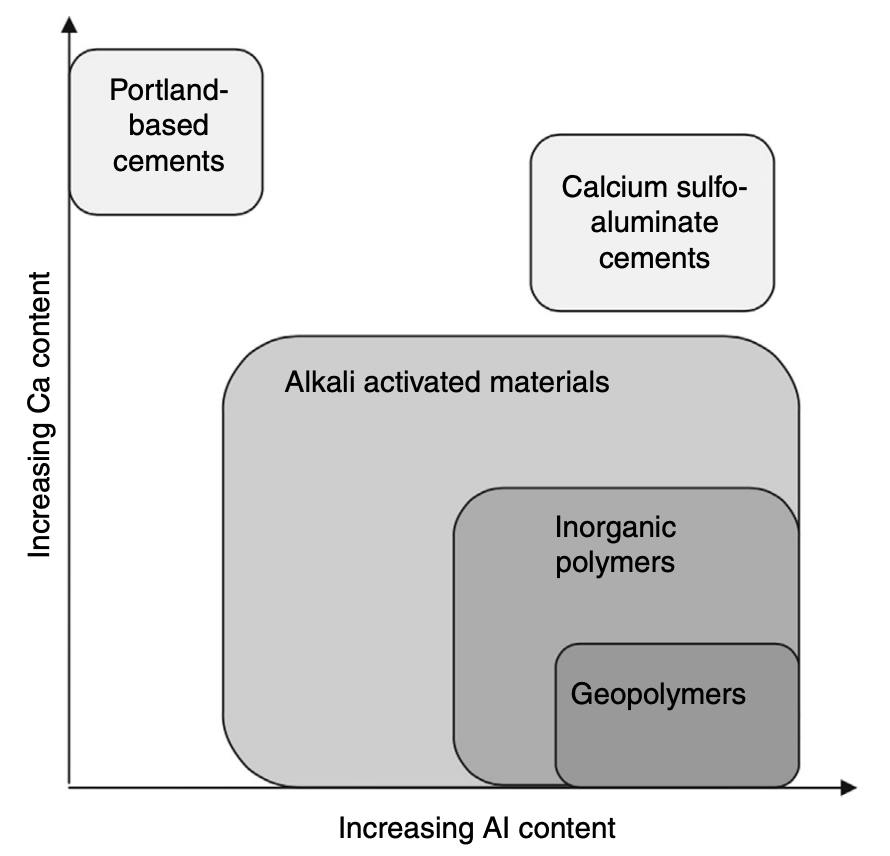
\includegraphics[width=0.5\textwidth]{Cap2/images/al_ca_aam.png}
  \caption{Classification of different subsets of alkali-activated
materials, with comparisons to Portland cement and
calcium sulfoaluminate binder chemistry. Shading
indicates approximate alkali content; darker shading
corresponds to higher concentrations of Na and/or K \cite{rakhimova2019reaction}.}
  \label{fig:al_ca_aam}
\end{figure}


\section{Raw Materials for AAM}

\subsection{Precursors}

Precursors are materials rich in $SiO_2$ and $Al_2O_3$ that, when activated by an alkaline solution, form a three-dimensional network of aluminosilicates \cite{rakhimova2019metakaolin}.
The mechanical and kinetic properties of AAMs are strongly influenced by the $SiO_2/Al_2O_3$ ratio \cite{provis2007geopolymerisation}.
The initial activation process involves the dissolution of aluminosilicates through the breaking of covalent bonds $Si-O-Si$ and $Al-O-Al$ in a high pH environment \cite{Severo2013}. Hydrolysis can be represented as follows:

\begin{equation}
  Al_2O_3 + 3H_2O + 2OH^- \rightarrow 2\left[Al(OH)_4\right]^- 
\end{equation}

\begin{equation}
  SiO_2 + H_2O + OH^- \rightarrow \left[SiO(OH)_3\right]^- 
\end{equation}

\begin{equation}
  SiO_2 + 2OH^- \rightarrow \left[SiO_2(OH)_2\right]^{2-}
\end{equation}

Subsequently, the dissolved silicates and aluminates react with each other, forming a gel that undergoes polymerization and hardening processes, as illustrated in Figure \ref{fig:activation}.

\begin{figure}[ht]
  \centering
  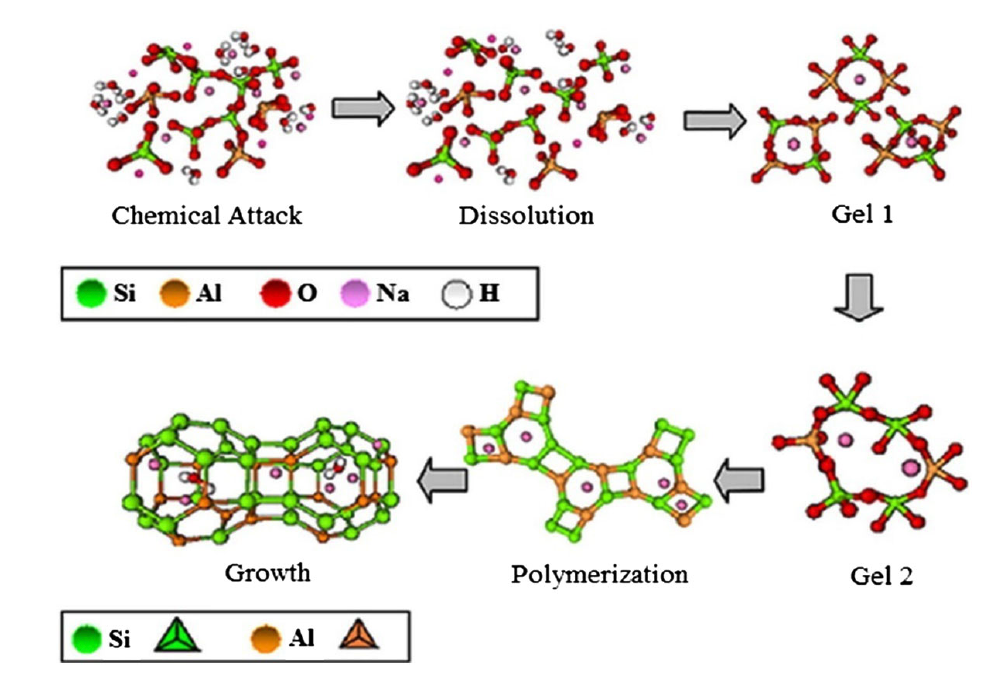
\includegraphics[width=0.75\textwidth]{Cap2/images/activation.png}
  \caption{Scheme of the alkaline activation process \cite{duxson2006geopolymer}.}
  \label{fig:activation}
\end{figure}

Precursors can be divided into two categories: those with high calcium content, such as blast furnace slag and fly ash, and those with low calcium content, such as metakaolin.
Figure \ref{fig:ternary_diagram} shows the most common precursors and their respective chemical compositions.

\begin{figure}[ht]
  \centering
  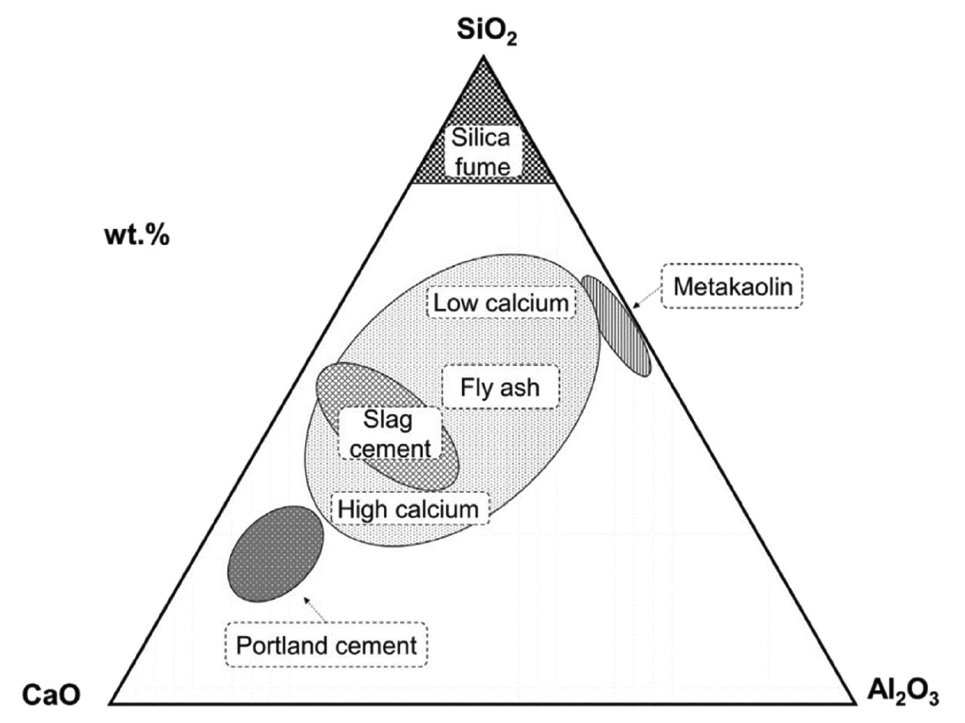
\includegraphics[width=0.625\textwidth]{Cap2/images/ternary_diagram.png}
  \caption{Ternary diagram of the most common precursors \cite{giergiczny2019fly}.}
  \label{fig:ternary_diagram}
\end{figure}

The first group primarily produces calcium aluminate silicate hydrate (C-A-S-H) as a result of the activation reaction, while the second group predominantly forms sodium aluminosilicate hydrate (N-A-S-H) gel.

When the calcium levels in these precursors are high, the final product is a gel with rapid curing and high initial strength. However, these systems are more susceptible to shrinkage, cracking, and corrosion due to chloride attack.
On the other hand, low-calcium systems form an tetrahedrical amorphous network, which exhibits low permeability and shrinkage, better fire resistance, and a less porous structure.
The $SiO_2/Al_2O_3$ ratio is responsible for the degree of polymerization of the formed gel; therefore, if the ideal ratio is not achieved, the mechanical strength and durability of the AAM may be compromised.
Finally, the N-A-S-H gel requires a longer curing time and a temperature between $80-100\ ^\circ C$ to reach the appropriate mechanical strength \cite{Nodehi2021}.

Table \ref{tab:common_precursors} presents the main characteristics of the most common precursors.

\begin{landscape}
\begin{table}[p]
  \centering
  \caption{Characteristics of common or innovative residual materials that can be added to concrete to produce more sustainable binders \cite{Nodehi2021}.}
  \vspace{0.5cm}
  {\small % Reduce font size for the table
  \renewcommand{\arraystretch}{1.2} % Increase row spacing
  \begin{tabular}{p{3.5cm} p{3cm} p{2cm} p{2cm} p{4cm} p{6cm}}
    \hline
    Additive name & Usual form & Average density (kg/m\textsuperscript{3}) & Average particle size (\textmu m) & Limitations & Benefits \\
    \hline
    Portland cement (OPC) & Irregular and angular & 1440 & 0.15--20 & -- & -- \\
    Silica fume & Spherical & 2200 & 0.1--0.5 & Reduces workability and initial strength & Increases compactness, mechanical strength, and durability \\
    Ground granulated blast furnace slag (GGBFS) & Angular with rough surface & 1000--1300 & 1.25--250 & Low initial strength & Increases durability, improves ITZ, and sulfate resistance \\
    Fly ash & Spherical & 540--860 & 0.5--300 & Low initial strength & Improves workability and long-term strength \\
    Metakaolin & Porous, lamellar, and angular & 890 & 1--20 & Reduces workability & Fills microstructure and improves ITZ \\
    Rice husk ash & Irregular with high porosity & 504--700 & 5--10 & Property variation and low reactivity & High silica content; improves compactness and strength \\
    Glass powder & Irregular & 2500 & 0.8--50 & High contamination & Improves durability and pozzolanic reaction \\
    Red mud & Irregular and needle-shaped & 2700--3400 & 100 to over 200 & High contamination & High alumina content, can improve hydration \\
    Ceramic waste & Angular & ~1700 & Below 100 & -- & Improves compactness and performance \\
    Municipal solid waste incineration slag (MSWI) & Irregular & 660--1690 & -- & -- & Improves microstructure and reduces porosity \\
    Paper sludge ash & Irregular & Below 100 & -- & -- & Favourably adjusts the S/A ratio \\
    \hline
  \end{tabular}
  }
\label{tab:common_precursors}
\end{table}
\end{landscape}

% \subsubsection{Metakaolin}

% \subsubsection{Silica Fume}

\subsection{Activators}

The alkaline attack on the microstructure of the precursors results in the release of silicates and aluminates into the solution.
The solubility of silica and alumina as a function of pH is presented in Figure \ref{fig:solubility}.

\begin{figure}[ht]
  \centering
  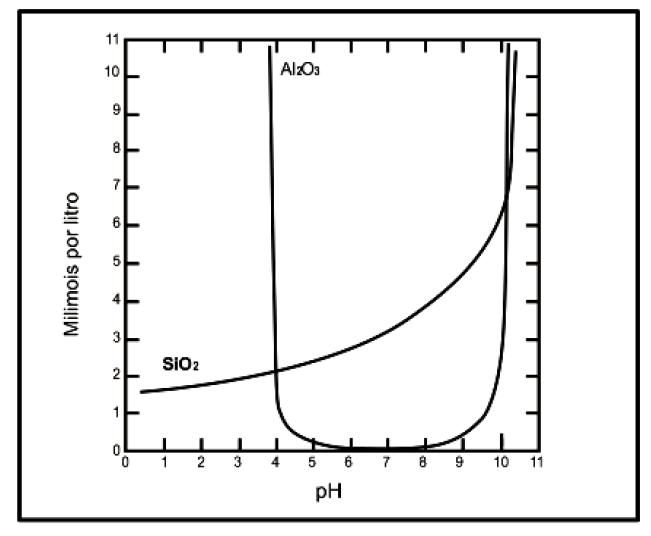
\includegraphics[width=0.625\textwidth]{Cap2/images/solubility.png}
  \caption{Solubility of silica and alumina as a function of pH \cite{mason1952principles}.}
  \label{fig:solubility}
\end{figure}

It is observed that the solubility of silica is low in acidic environments and high in basic media, while alumina is soluble at both extremes of pH.
Therefore, for the activation reactions to occur, it is necessary that the pH of the solution is high.

Alkaline activators can be found in two forms: liquid—producing two-part geopolymers—or solid—one-part geopolymers.
The main liquid alkaline activators are: sodium hydroxide ($NaOH$), sodium silicate ($Na_2SiO_3$), potassium hydroxide ($KOH$), sodium carbonate ($Na_2CO_3$), potassium carbonate ($K_2CO_3$), and potassium oxide ($K_2O$).
The first studies on AAM focused on liquid activators, since the final product exhibits high compressive strength, adhesion, and the ability to withstand fatigue loads. In addition, they also demonstrate high resistance to freeze-thaw cycles and high temperatures \cite{heath2014gwp}.

Despite the advantages of two-part systems, basic solutions are corrosive and irritate human skin, making their transport and handling hazardous for workers \cite{awoyera2019critical}.
Another point worth noting is that the production of sodium silicate occurs between $1200-1400\ ^\circ C$ and emits approximately 1.514 kg of $CO_2$ per kg of silicate produced, in addition to significantly contributing to air pollution through dust and nitrogen and sulfur oxides \cite{rajan2020sustainable}.


%% Antes de falar que é menos perisogoso e mais ecalável, falar dos downsizes de propriedades mecanicas e curaa térmica
Thus, one-part systems emerge as a safer alternative, since solid activators are less hazardous and easier to handle. Even though one-part geopolymers exhibit lower mechanical strength and require thermal curing to achieve adequate performance \cite{provis2018alkali}, their use is more scalable.

\section{Environmental Impacts}

The main environmental advantage attributed to AAMs lies in the considerable reduction of $CO_2$ emissions compared to traditional Portland cement.
It is estimated that the environmental impacts of solid and liquid activators are 24\% and 60\% of the impact caused by OPC, respectively \cite{luukkonen2017review}.
Furthermore, the production of AAMs often utilizes industrial residues as raw materials, such as blast furnace slag, sewage sludge ash, rice husk ash, sugarcane straw ash, among others \cite{moraes2024scsa}.
Therefore, in addition to the valorization of industrial waste, the production of AAMs reduces the demand for natural resources from mineral deposits and provides an environmentally appropriate destination, following the guidelines of the National Solid Waste Policy \cite{PNRS2016}.

\section{Mechanical Properties}



\chapter{Methodology}
\section{Materials}
\label{sec:materials}

For the development of one-part geopolymeric pastes and mortars, the following components were used:

\begin{itemize}
    \item Caolin supplied by the company Brasilminas;
    \item Silica fume (SF) supplied by the company Elken;
    \item Potassium carbonate supplied by the company Neon (purity of 98\%);
    \item Calcium hydroxide supplied by the company Neon  (purity of 95\%);
    \item Standardized quartz sand supplied by the company IPT;
    \item Distilled water.
\end{itemize}

The precursors used were silica fume and metakaolin. However, the purity of commercially available metakaolin is not sufficient to ensure precision in the characterization of cementitious samples.
Therefore, it was produced from commercial kaolin, as detailed in Section \ref{sec:production_of_metakaolin}.
The alkaline sources are commercially available with high purity, so the physicochemical compositions provided by the manufacturer were used.

% The chemical composition of the materials used in the formulation of the mortars is presented in Table \ref{tab:chemical_composition_reagents}.
% 
% \begin{table}[H]
%     \caption{Chemical properties of the solid reagents.}
%     \label{tab:chemical_composition_reagents}
%     \center
%     \begin{tabular}{ccc}
%         \hline
%         Material & Chemical composition & Specification (\%)\\
%         \hline
%         Silica fume & $SiO_2$ &  \textcolor{red}{XX,X} \\
%             & $ Al_2O_3$ & \textcolor{red}{XX,X} \\
%             & $MgO$ & \textcolor{red}{XX,X} \\
%             & $CaO$ & \textcolor{red}{XX,X} \\
%             & $Fe_2O_3$ & \textcolor{red}{XX,X} \\
%         Potassium carbonate & $K_2CO_3$ & \textcolor{red}{XX,X} \\
%         Calcium hydroxide & $Ca(OH)_2$ & \textcolor{red}{XX,X} \\
%         \hline
%     \end{tabular}
% \end{table}

In addition, the quartz sand used follows the standards established by the Institute for Technological Research (IPT), as shown in Tables \ref{tab:quartz_sand_properties} and \ref{tab:quartz_sand_granulometry}.

\begin{table}[H]
    \caption{Results of physical and chemical requirements of standardized quartz sand.}
    \label{tab:quartz_sand_properties}
    \center
    \begin{tabular}{p{0.30\textwidth} p{0.25\textwidth} p{0.25\textwidth}}
        \hline
        Property & Result & ABNT NBR7214:2015 Requirement\\
        \hline
        Silica content (ABNT NBR14656:2001) & 96.5\% & $\geq$ 95\%, by mass \\
        Moisture (ABNT NBR7214:2015) & 0.0\% & $\leq$ 0.2\%, by mass \\
        Organic matter (ABNT NBR17053:2022) & Lighter or equal to the color of the standard solution & Color of the 2\% tannic acid standard solution \\
        \hline
    \end{tabular}
\end{table}

\begin{table}[H]
    \caption{Particle size distribution of the fractions of standardized quartz sand.}
    \label{tab:quartz_sand_granulometry}
    \centering
    \begin{tabular}{p{0.10\textwidth} p{0.30\textwidth} p{0.15\textwidth} p{0.25\textwidth}}
        \hline
        \multirow{2}{*}{Fraction} & \multirow{2}{*}{Sieve interval} & \multicolumn{2}{c}{Mass percentage (\%)} \\ \cline{3-4}       
        & & Result & ABNT NBR7214:2015 Requirement\\
        \hline
        16 & (2.4 mm and 2.0 mm) & 0 & $\leq$ 10 \\
        16 & (2.0 mm and 1.2 mm) & 97 & $\geq$ 90 \\
        30 & (1.2 mm and 0.6 mm) & 99 & $\geq$ 95 \\
        50 & (0.6 mm and 0.3 mm) & 96 & $\geq$ 95 \\
        100 & (0.3 mm and 0.15 mm) & 95 & $\geq$ 95 \\
        \hline
    \end{tabular}
\end{table}

\section{Methods}
\label{sec:methods}
The experimental process was divided into three steps: (i) production and characterization of raw-materials; (ii) production of geopolymeric pastes and mortars; (iii) microstructural studies and mechanical tests of hardened state.

\subsection{Production and Characterization of Raw Materials}
\label{sec:production_characterization_raw_materials}

\subsubsection{Production of Metakaolin}
\label{sec:production_of_metakaolin}

Metakaolin was obtained by calcining kaolin at $700\ ^\circ C$ for 1 hour in a 200 L 18 kW laboratory furnace.
The optimal calcination time and temperature were determined from preliminary tests, in which the yield of calcination and reactivity was evaluated.
To ensure material homogeneity, two shallow trays with a maximum height of 10 mm were used.
The transformation of crystalline kaolinite into amorphous metakaolinite is represented by Equation \ref{eq:calcination_kaolin}.

\begin{equation}
    \label{eq:calcination_kaolin}
        Al_2.Si_2O_5\left(OH\right)_4 \xrightarrow{\Delta} Al_2O_3.2SiO_2 + 2 H_2O
\end{equation}

\subsubsection{Physicochemical Characterization of Solid Precursors}
\label{sec:physicochemical_characterization_precursors}

The physicochemical characterization of the solid precursors was carried out at the laboratories of the Aeronautics Institute of Technology (ITA), located in São José dos Campos-SP.

To  verify the removal of hydroxyl groups ($OH^-$) was verified by loss on ignition (LOI).
In addition, X-ray diffraction (XRD) was used to determine the crystalline phase of metakaolin and silica fume.
XRD was performed by a Panalytical Empyrean diffractometer, with a $2\theta$ interval of $10$-$70^\circ$, Cu-$\mathrm{K}\alpha$ radiation, $0.01^\circ$ step and 50 s/step.


% As distribuições granulométricas do metacaulim (MC), escória de alto forno (EAF) e sílica ativa (SA) foram determinadas por difração a LASER, utilizando-se um equipamento CILAS1090. As amostras foram dispersas em água destilada, e as condições de ensaio adotadas incluíram agitação a 1500 rpm, tempo de ultrassom de 2,5 minutos, obscuração entre 10 e 20%, e tempo total de dispersão de 5 minutos.
Finally, the particle size distribution (PSD) of the solids used was determined by laser diffraction. Smaller and more irregular particles tend to have a higher specific surface area and, therefore, greater reactivity in contact with the alkaline source, which can directly influence the mechanical performance and rheological properties of the geopolymeric mortars.
PSD was analyzed in a Malvern Mastersizer 3000 particle size analyzer, with air as the dispersion agent, at 1.5 bar pressure and a 40\% feed rate.

\subsection{Production of Geopolymeric Pastes and Mortars}
\label{sec:production_geopolymeric_pastes_mortars}

\subsubsection{Mix Design}
\label{sec:mix_design}

The development of one-part geopolymeric mortars followed a systematic experimental design, aiming to evaluate the effect of different compositions on physicochemical and mechanical properties.

The variables considered in the study were:

\begin{itemize}
    \item Proportion between solid precursors (metakaolin and silica fume);
    \item Content of alkaline activators ($K_2CO_3$ and $Ca(OH)_2$);
    \item Water/solids ratio (w/s);
    \item Sand/binder ratio (s/b).
\end{itemize}

The variable of interest in this experiment is the $Si/Al$ ratio, which will be varied from 1.0 to 5.0, calculated based on the proportion of metakaolin and silica fume.

Initially, the water/solids ratio was determined %analogously to \textcolor{red}{ref xxxx}, 
by ensuring adequate workability of the pastes.

In addition, due to stoichiometric balance, the $Al/K$ ratio will be constant and equal to 1, according to the empirical formula on Equation \ref{eq:al_k_ratio} \cite{joseph1991geopolymers}, where $M$ is a sodium or potassium cation.

\begin{equation}
    \label{eq:al_k_ratio}
    M_n \left\{ \left(SiO_2 \right)_z AlO_2 \right\}_n \cdot wH_2O
\end{equation}

Furthermore, the $K/Ca$ ratio will be constant and equal to 2, respecting the precipitation reaction of potassium carbonate with calcium hydroxide, as shown in Equation \ref{eq:k_ca_reaction}.

\begin{equation}
    \label{eq:k_ca_reaction}
    K_2CO_3 + Ca(OH)_2 \rightarrow  2KOH_{(aq)} + CaCO_{3(s)} \downarrow
\end{equation}

With the paste proportions well defined, the production of mortars maintained a 1:2 ratio between binder and sand, analogously in the previous researches \cite{batista2025mgosio2}. 

Table \ref{tab:mortar_compositions} presents the different formulations produced, with the respective mass proportions of the components.

\begin{table}[H]
    \caption{Compositions of the produced geopolymeric mortars.}
    \label{tab:mortar_compositions}
    \center
    \begin{tabular}{cccccccc}
        \hline
        Sample & \multicolumn{2}{c}{Precursors (\%)} & \multicolumn{2}{c}{Activators (\%)} & \multirow{2}{*}{w/s} & \multirow{2}{*}{s/b} & \multirow{2}{*}{Si/Al} \\
        \cline{2-5}
        & MK & SF & $K_2CO_3$ & $Ca(OH)_2$ & & & \\
        \hline
        A1 & \textcolor{red}{XX} & \textcolor{red}{XX} & \textcolor{red}{X,X} & \textcolor{red}{X,X} & \textcolor{red}{X,XX} & 2 & \textcolor{red}{1,0} \\
        A2 & \textcolor{red}{XX} & \textcolor{red}{XX} & \textcolor{red}{X,X} & \textcolor{red}{X,X} & \textcolor{red}{X,XX} & 2 & \textcolor{red}{2,0} \\
        A3 & \textcolor{red}{XX} & \textcolor{red}{XX} & \textcolor{red}{X,X} & \textcolor{red}{X,X} & \textcolor{red}{X,XX} & 2 & \textcolor{red}{3,0} \\
        A4 & \textcolor{red}{XX} & \textcolor{red}{XX} & \textcolor{red}{X,X} & \textcolor{red}{X,X} & \textcolor{red}{X,XX} & 2 & \textcolor{red}{4,0} \\
        A5 & \textcolor{red}{XX} & \textcolor{red}{XX} & \textcolor{red}{X,X} & \textcolor{red}{X,X} & \textcolor{red}{X,XX} & 2 & \textcolor{red}{5,0} \\
        \hline
    \end{tabular}
\end{table}

\subsubsection{Mixing Procedure}
\label{sec:mixing_procedure}

The production of the mixtures followed standardized procedures. For the production of mortars and compressive strength testing, the procedures of the Brazilian standard \cite{ABNT_NBR_7215_2019} were followed. For the production of pastes, the American standard \cite{ASTM_C305_2006} was chosen, since the Brazilian standard does not specify the mixing procedure for cementitious pastes without fine aggregate. Both procedures were adapted for the preparation of small-volume samples.

\subsubsection{Molding and Curing of Specimens}
\label{sec:molding_and_curing_specimens}

For the compressive strength test, the specimens were prepared in prismatic molds with dimensions $40 \times 40 \times 40 \ mm$, previously lubricated with oil-based release agent.

For each composition, 9 specimens were molded, intended for testing at ages of 1, 3, and 7 days (3 specimens for each age). It was not necessary to perform tests at 28 days, as the thermal curing of the binders used provides high initial strength gain.
% , as demonstrated in the literature \textcolor{red}{ref XXX}.

Thermal curing was carried out in an oven maintained at (60 ± 2)°C and a minimum relative humidity of 95\% for 24 hours, as recommended by the standard \cite{ABNT_NBR_9479_2006}, to ensure the activation of the binders and accelerate the curing process.
It is noteworthy that demolding was performed 24 hours after the start of the curing process.

Demolding was performed 24 hours after molding, and the specimens were immediately transferred to the corresponding curing conditions until the testing age.

For microstructural analyses, small samples were separated, with hydration interrupted by immersion in ethyl alcohol and vacuum filtration, followed by drying in an oven at 40°C for 24 hours.
%% EXPLICAR PQ ALcool
% The alcohol was used to prevent rehydration of the samples, as it is a dehydrating agent that does not react with the components of the geopolymeric paste.
These samples were stored in hermetically sealed containers to prevent rehydration.

\subsection{Microstructural studies and Mechanical tests of hardened state}
\label{sec:microstructural_studies_mechanical_tests_hardened_state}

\section{Characterization of Geopolymeric pastes}
\label{sec:characterization_geopolymeric_pastes}

Energy-dispersive X-ray spectroscopy (EDS) was used to determine the proportion of chemical elements, performed together with scanning electron microscopy (SEM) to evaluate the morphology of the solid precursors.
SEM/EDS was performed using a TESCAN VEGA 3 XMU device and Oxford EDS 133 eV detector, with gold coated.

To verify the presence of $Al-Si-O$ bonds, Fourier-transform infrared spectroscopy (FTIR) was carried out in a PerkinElmer spectrophotometer, with a spectrum range of $4000$–$400\ cm^{-1}$ and a spectral resolution of $1\ cm^{-1}$.
Moreover, XRD and PSD were performed under the same conditions applied for the raw materials.

Lastly, the total porosity and pore size distribution of the hardened pastes were determined by mercury intrusion porosimetry (MIP).

\subsubsection{Compressive Strength of mortars}
\label{sec:compressive_strength}

For the compressive strength test, the specimens were placed in a hydraulic press with  a 600 kN-load limit, applying load at a rate of 0.5 kN/s until failure. The strength was calculated by the equation:

\begin{equation}
    \label{eq:compressive_strength}
    R_c = \frac{F_c}{A_t}
\end{equation}

Where:
\begin{itemize}
    \item $R_c$ is the compressive strength, in MPa;
    \item $F_c$ is the maximum applied load, in N;
    \item $A_t$ is the cross-sectional area, in mm\textsuperscript{2}.
\end{itemize}

For statistical analysis, the Tukey test was performed, allowing the identification of significant differences between sample groups, considering a significance level of 95\%.

% \subsection{Microstructural Analyses}
% \label{sec:microstructural_analyses}

% \subsubsection{X-ray Diffraction (XRD)}
% \label{subsec:xrd}

% X-ray diffraction analyses were performed on ground paste samples with particle size less than 75 µm, at ages of 7 and 28 days. A diffractometer from \textcolor{red}{XXX}, model \textcolor{red}{XXX}, was used.
% %  with copper radiation (Cu-Kα, λ = 1.5418 Å), operating at 40 kV and 30 mA. Scans were performed at an angular speed of 0.02° per second, in a range from 5° to 80° (2θ).

% \subsubsection{Fourier Transform Infrared Spectroscopy (FTIR)}
% \label{subsec:ftir}

% Infrared spectroscopy was performed on ground paste samples with particle size less than 45 µm, at ages of 1, 3, and 7 days. A spectrometer from \textcolor{red}{XXX}, model \textcolor{red}{XXX}, was used, in the range of \textcolor{red}{XXX} to \textcolor{red}{XXX} cm$^{-1}$, with a resolution of \textcolor{red}{XXX} cm$^{-1}$ and \textcolor{red}{XXX} scans.

% \subsubsection{Scanning Electron Microscopy (SEM)}
% \label{subsec:sem}

% The microstructural analysis of the pastes was performed by scanning electron microscopy, using a microscope from \textcolor{red}{XXX}, model \textcolor{red}{XXX}, coupled to an energy-dispersive X-ray spectrometer (EDS). The samples were prepared from cylindrical fragments of pastes molded in a disposable plastic straw.
% % Analyses were performed at magnifications of 500×, 2000×, and 5000×, with an acceleration voltage of 15 kV.



\chapter{Results and Discussion}
\section{Chemical and Physical Characterization of Precursors}
\label{sec:chemical_and_physical_characterization_of_precursors}

\subsection{Chemical Composition of Precursors}
\label{sec:chemical_composition_of_precursors}

The chemical composition of the aluminosilicate precursors plays a fundamental role in determining their reactivity and suitability for activation in a low-calcium system. 
In this work, the metakaolin (MK) and silica fume (SF) precursors were analysed for their oxide content (normalized with respect to the powder fraction) and loss on ignition (LOI), which was found to be 0.69\% and 2.27\%, respectively.
% The results are presented in Table \ref{tab:mk_sa_composition}.

\begin{table}[H]
    \centering
    \caption{Chemical composition (wt \%) of the precursors: metakaolin (MK) and silica fume (SF).}
    \label{tab:mk_sa_composition}
    \begin{tabular}{l c c c c}
        \hline
        \multicolumn{1}{c}{Oxide} & \multicolumn{2}{c}{Metakaolin} & \multicolumn{2}{c}{Silica Fume} \\
        \cline{2-5}
        & wt (\%) & wt with LOI (\%) & wt (\%) & wt with LOI (\%) \\
        \hline
        K\textsubscript{2}O & 0.21 & 0.20 & 0.74 & 0.73 \\
        CaO & 0.19  & 0.19 & 0.13 & 0.13 \\
        MgO & 2.60 & 2.59 & 0.00 & 0.00 \\
        P\textsubscript{2}O\textsubscript{5} & 0.00 & 0.00 & 0.00 & 0.00 \\
        Cl & 0.00 & 0.00 & 0.12 & 0.12 \\
        SO\textsubscript{3} & 0.00 & 0.00 & 0.15 & 0.15 \\
        SiO\textsubscript{2} & 49.37 & 49.03 & 96.90 & 94.70 \\
        Fe\textsubscript{2}O\textsubscript{3} & 0.77 & 0.76 & 1.78 & 1.74 \\
        Al\textsubscript{2}O\textsubscript{3} & 46.38 & 46.06 & 0.00 & 0.00 \\
        Na\textsubscript{2}O & 0.00 & 0.00 & 0.17 & 0.17 \\
        TiO\textsubscript{2} & 0.49 & 0.48 & 0.00 & 0.00 \\
        \hline
    \end{tabular}
\end{table}

From Table 4.1.1 it is clear that the MK precursor is rich in alumina and contains a significant silica fraction , while the SA is extremely high in silica and essentially alumina-free.
Critically, both materials present very low CaO contents.
The minimal presence of calcium oxide is an important indicator of the low-calcium nature of the precursors, which is a pre-requisite for favoring the formation of potassium aluminosilicate hydrate type gels, rather than calcium-rich gels, as often observed when using ground granulated blast furnace slag \cite{ali2023geopolymer}.


In addition, the low LOI values suggest a limited amount of residual organics or volatile components, which could otherwise interfere with the dissolution kinetics of the aluminosilicates.
Furthermore, the Si/Al molar ratio of MK precursos is approximately 0.9, which will be used with the essentially pure SA to tailor the mix designs for optimal geopolymerization reactions, as presented in Appendix \ref{appendix:mix_designs}.

% Create a slide with this phrase:
In summary, the chemical data confirm that both MK and SA meet the key requirements of (i) high silica and/or alumina content, (ii) low calcium content, and (iii) minimal impurities, thereby validating their use as raw materials for a low calcium alkali-activated binder system.

\subsection{X-Ray Diffraction of Precursors and Alkaline Sources}
\label{sec:x-ray_diffraction_of_precursors_and_alkaline_sources}

XRD analysis was conducted on the precursors and alkaline sources to evaluate phase composition, crystallinity and the presence of amorphous phases. The key observations were as follows:

\begin{table}[H]
    \centering
    \caption{Summary of XRD phase observations for precursors and alkaline sources.}
    \label{tab:precursor_xrd_summary}
    \begin{tabular}{l l}
        \hline
        Material & Key XRD observations \\
        \hline
        MK & Broad amorphous hump near $2\theta \approx 21\degree$, residual quartz peaks (COD 900-9667) \\
        SA & Broad amorphous hump near $2\theta \approx 22.5\degree$, no distinct crystalline phases \\
        Ca(OH)\textsubscript{2} & Crystalline portlandite phase (COD 900-0114) \\
        K\textsubscript{2}CO\textsubscript{3} & Crystalline calcium carbonate phase (COD 900-9644) \\
        \hline
    \end{tabular}
\end{table}

SA and MK both exhibited broad amorphous humps in their XRD patterns, indicative of their largely non-crystalline nature, which is favorable for dissolution during alkali activation.
The MK showed minor crystalline quartz peaks, indicating the presence of impurities, which remains inert during calcination \cite{provis2014geopolymers} and acts as filler without participating in geopolymerization reaction \cite{rakhimova2019metakaolin}.
The alkaline sources displayed sharp diffraction peaks corresponding to their known crystalline phases, confirming their purity.

% \subsection{Fourier Transform Infrared Spectroscopy of Precursors}

% FTIR spectra of MK and SA precursors provided insights into their molecular structures and functional groups relevant to geopolymerization.


\section{Microstructural Characterization of Pastes}

\subsection{Scanning Electron Microscopy and Energy Dispersive Spectroscopy}

Scanning electron microscopy of the pastes cured for 3 days revealed a clear dependence of matrix morphology on the Si/Al molar ratio
At Si/Al ratio of 0.9, the SEM images of the paste showed a higher frequency of visibly unreacted precursor particles, together with needle-shaped crystalline features and larger pores. Those unreacted particles are likely some alkali carbonate products that precipitate when mobile alkalis are not fully incorporated into the aluminosilicate gel and subsequently react with atmospheric CO\textsubscript{2} \cite{provis2018alkali}.

\begin{figure}[H]
  \centering
  \subfloat[1000× magnification]{
    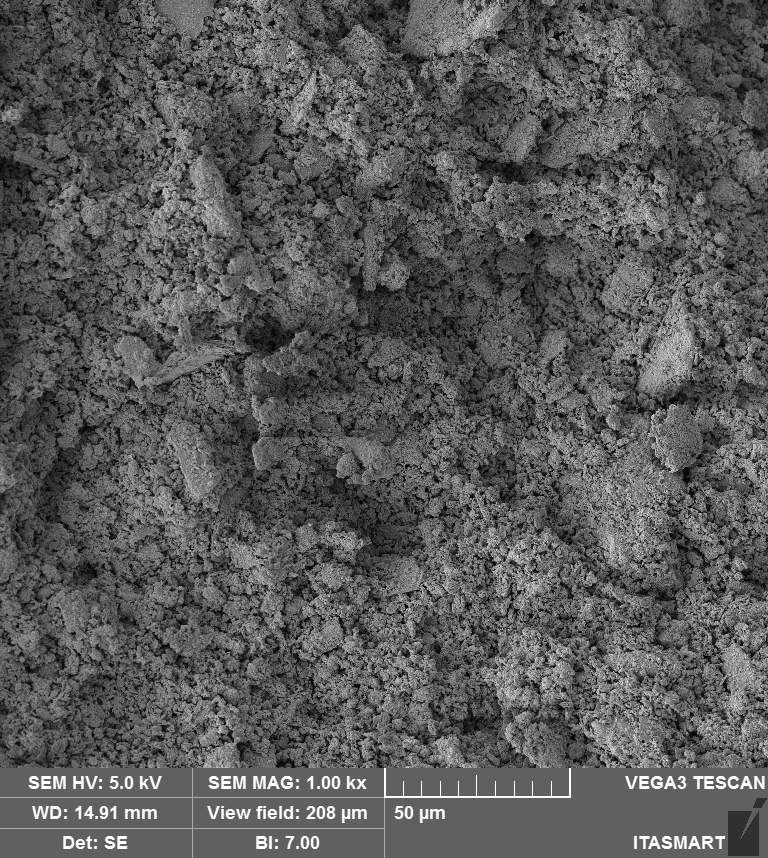
\includegraphics[width=0.4\textwidth]{Cap4/images/si_al_0-9_spot5_1000x.png}
    \label{fig:si_al_0-9_spot5_1000x}
  }
%   \hfill
  \subfloat[5000× magnification]{
    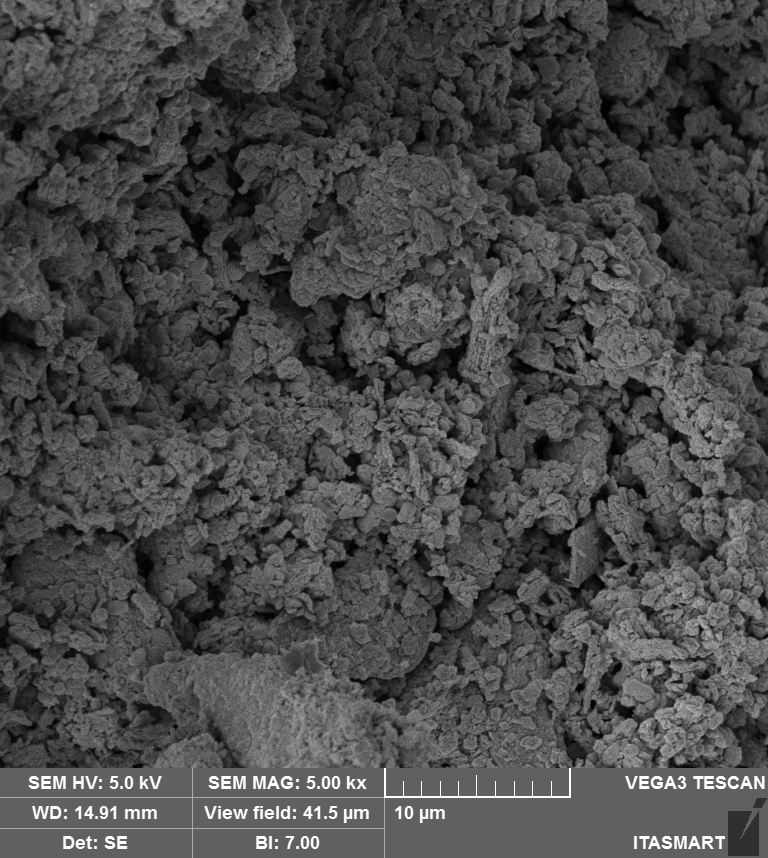
\includegraphics[width=0.4\textwidth]{Cap4/images/si_al_0-9_spot5_5000x.png}
    \label{fig:si_al_0-9_spot5_5000x}
  }
  \caption{SEM micrographs of paste with Si/Al = 0.9 after 3 days of curing (spot 5).}
  \label{fig:si_al_0-9_spot5}
\end{figure}

By contrast, the Si/Al ratio of 3.0 paste exhibited the densest and most homogeneous matrix, with fewer discernible unreacted particles and a more continuous binder phase.
This indicates that intermediate Si/Al values promote better network polymerization and denser structure.

\begin{figure}[H]
  \centering
  \subfloat[1000× magnification]{
    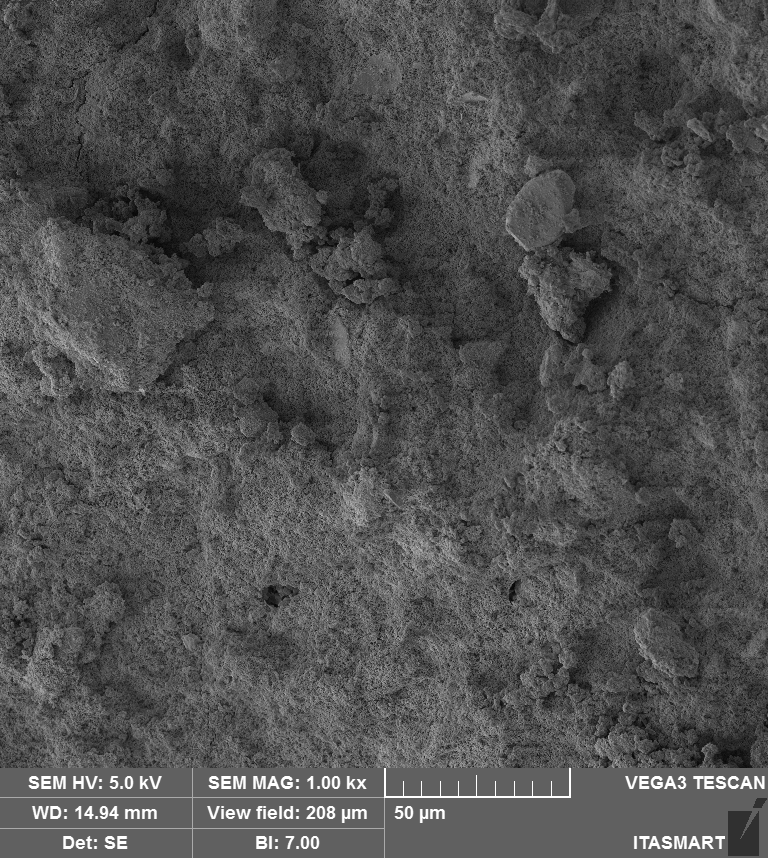
\includegraphics[width=0.4\textwidth]{Cap4/images/si_al_3-0_spot3_1000x.png}
    \label{fig:si_al_3-0_spot3_1000x}
  }
%   \hfill
  \subfloat[5000× magnification]{
    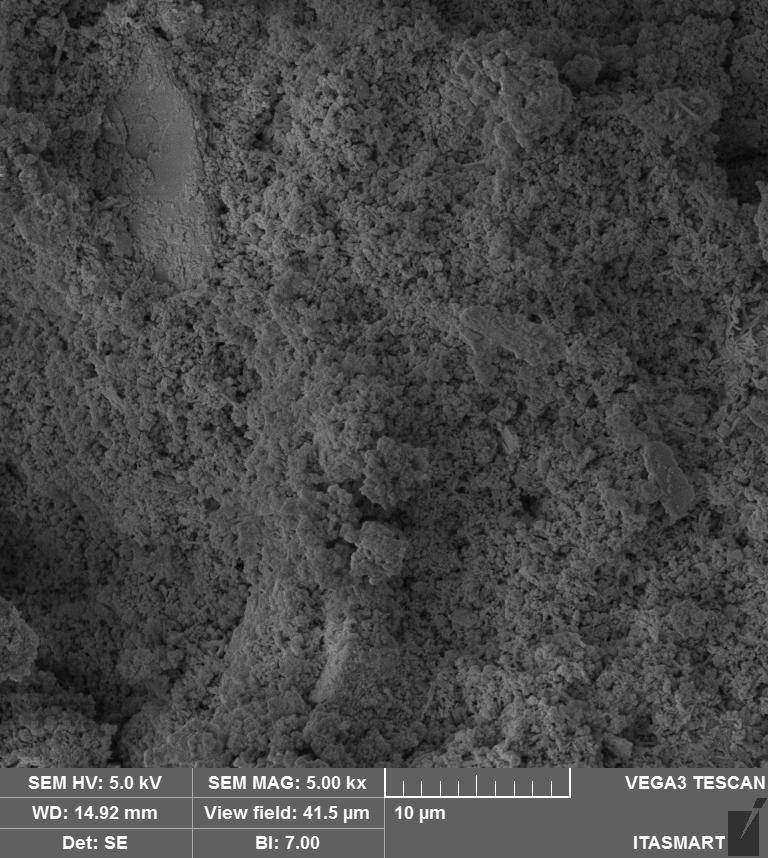
\includegraphics[width=0.4\textwidth]{Cap4/images/si_al_3-0_spot3_5000x.png}
    \label{fig:si_al_3-0_spot3_5000x}
  }
  \caption{SEM micrographs of paste with Si/Al = 3.0 after 3 days of curing (spot 3).}
  \label{fig:si_al_3-0_spot3_sem}
\end{figure}

At Si/Al = 5.0, the SEM images showed residual spherical particles characteristic of silica fume that were not fully reacted after the curing time, indicating that at very high Si/Al the silica supply exceeds the polymerization capacity of the system.


\begin{figure}[H]
  \centering
  \subfloat[1000× magnification]{
    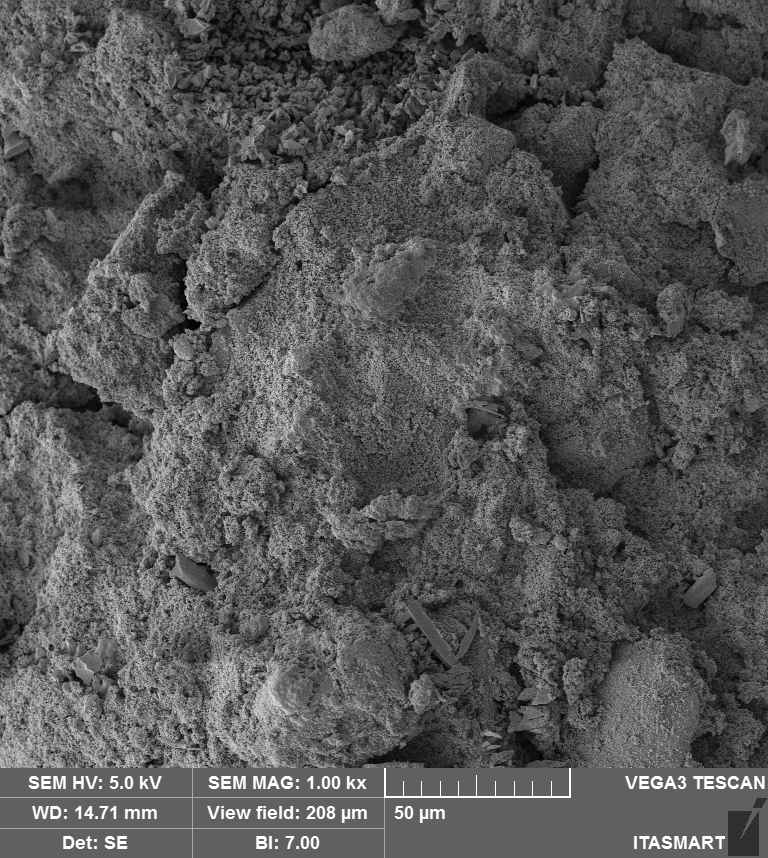
\includegraphics[width=0.4\textwidth]{Cap4/images/si_al_5-0_spot1_1000x.png}
    \label{fig:si_al_5-0_spot1_1000x}
  }
%   \hfill
  \subfloat[5000× magnification]{
    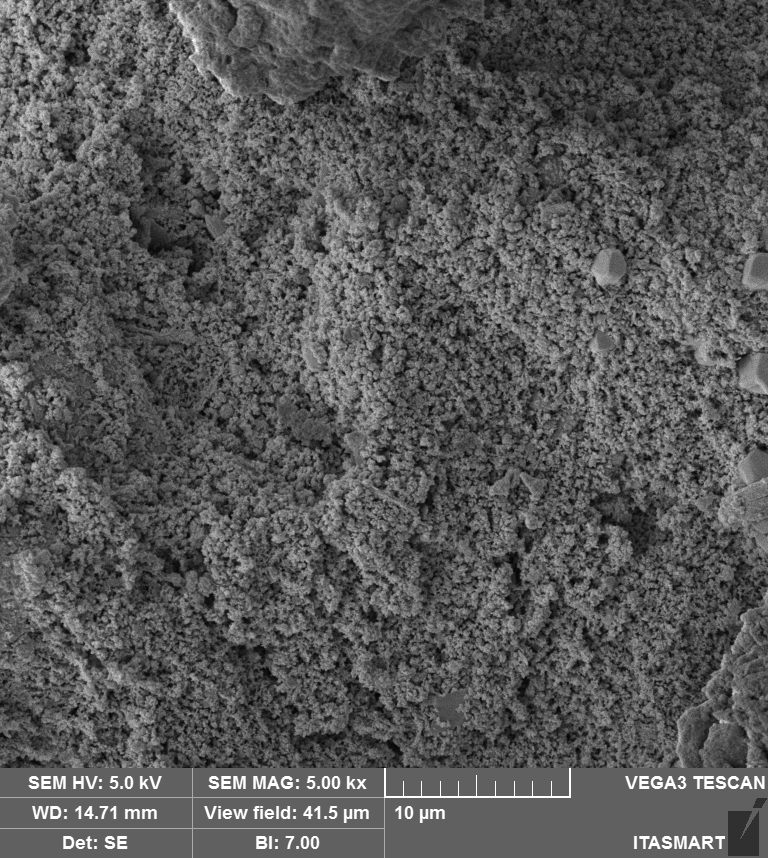
\includegraphics[width=0.4\textwidth]{Cap4/images/si_al_5-0_spot1_5000x.png}
    \label{fig:si_al_5-0_spot1_5000x}
  }
  \caption{SEM micrographs of paste with Si/Al = 5.0 after 3 days of curing (spot 1).}
  \label{fig:si_al_5-0_spot1_sem}
\end{figure}

The remaining pictures from SEM analysis are presented in Appendix \ref{appendix:sem_images}.

Energy dispersive spectroscopy was performed at representative gel regions and crystalline features observed in the SEM images.

\begin{figure}[H]
    \centering
    \subfloat[EDS layered image]{
        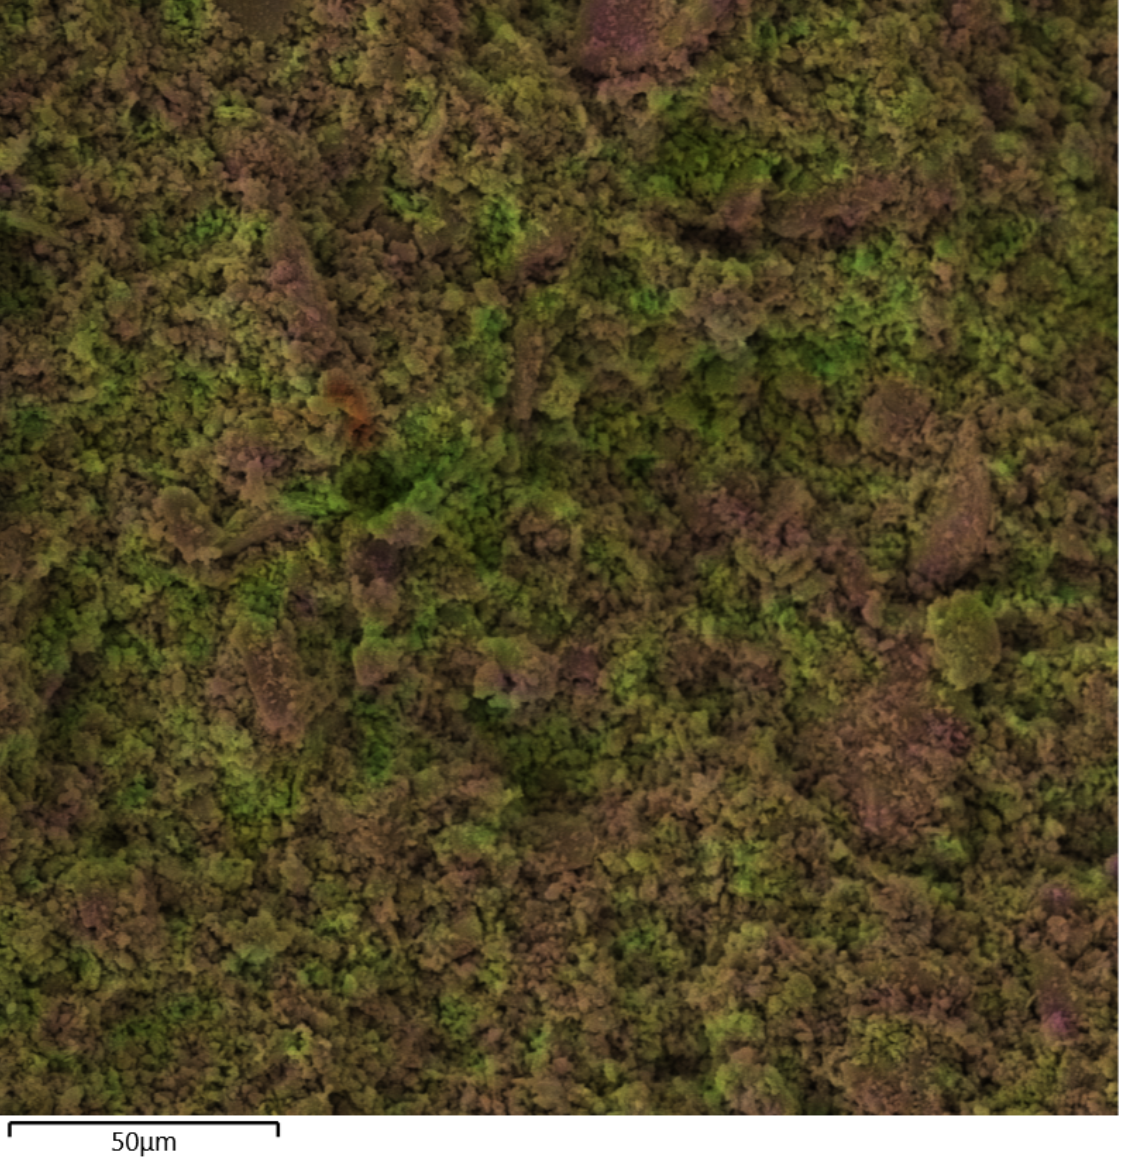
\includegraphics[height=6cm]{Cap4/images/0-9-60C-3d-Spot 5 - layered.png}
    }
    \hfill
    \subfloat[EDS map]{
        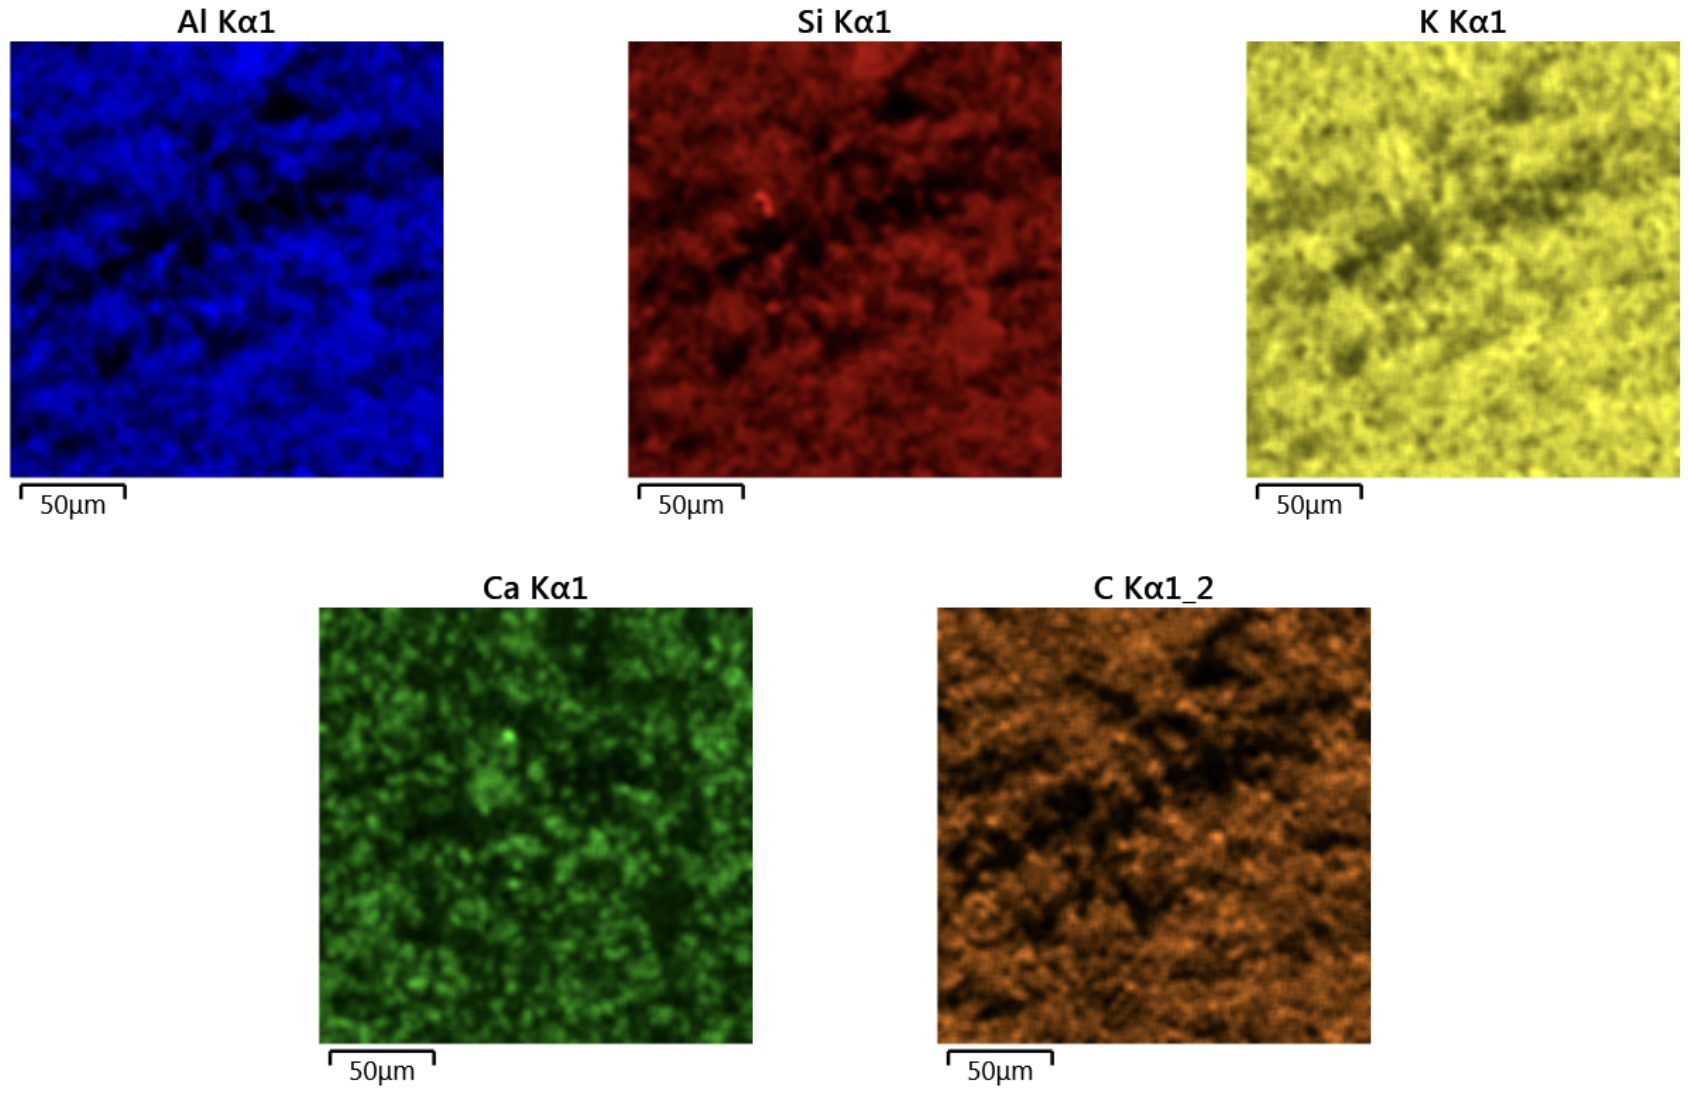
\includegraphics[height=6cm]{Cap4/images/0-9-60C-3d-Spot 5 - map.png}
    }
    \caption{EDS analysis of Spot 5, Si/Al = 0.9, cured for 3 days at 60°C at 1000× magnification.}
    \label{fig:eds_spot5_0-9}
\end{figure}

\begin{figure}[H]
    \centering
    \subfloat[EDS layered image]{
        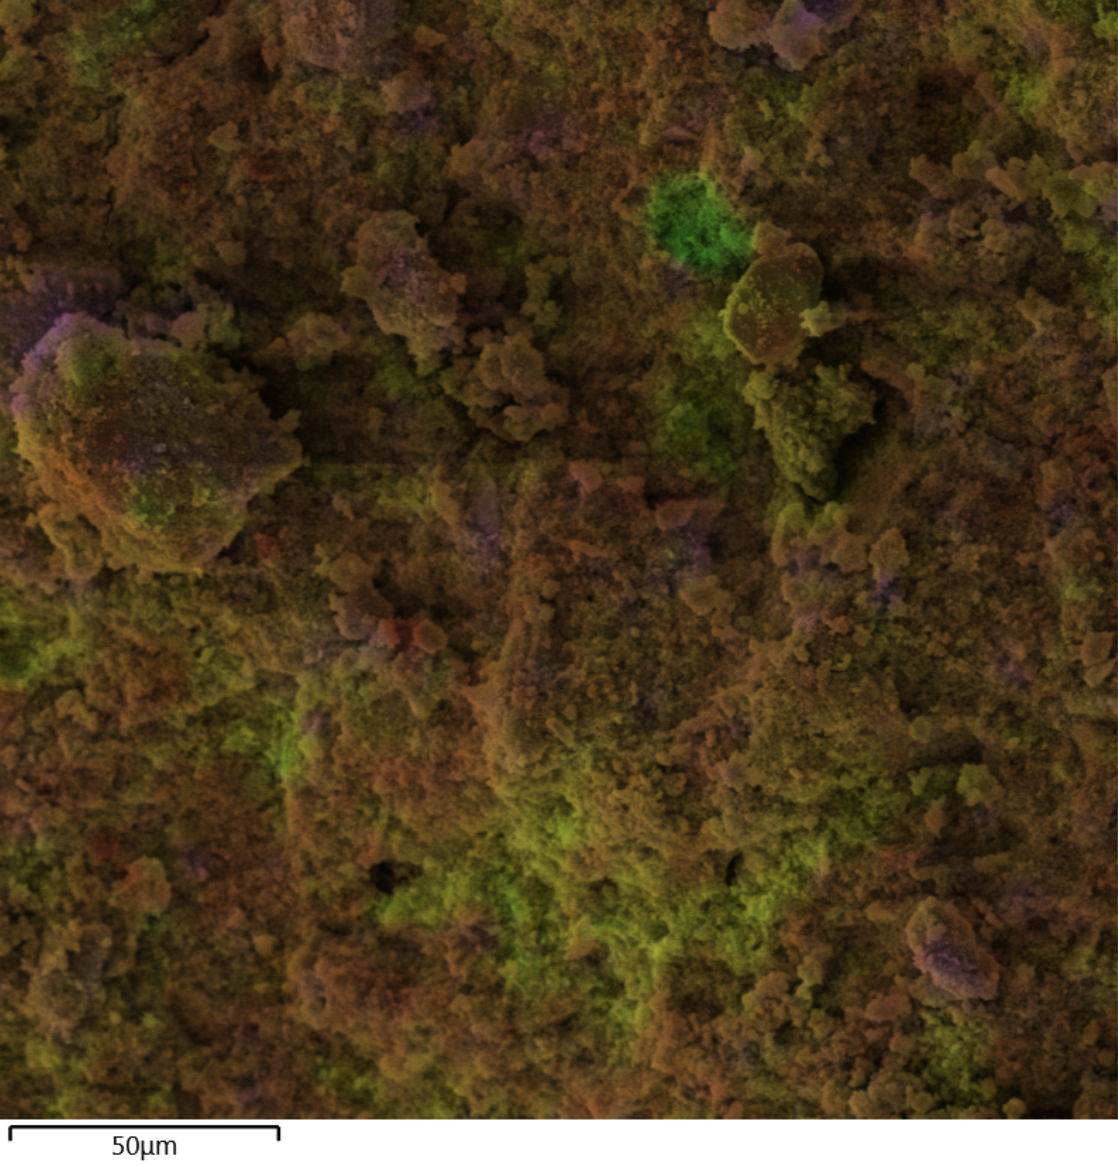
\includegraphics[height=6cm]{Cap4/images/3-0-60C-3d-Spot 3 - layered.png}
    }
    \hfill
    \subfloat[EDS map]{
        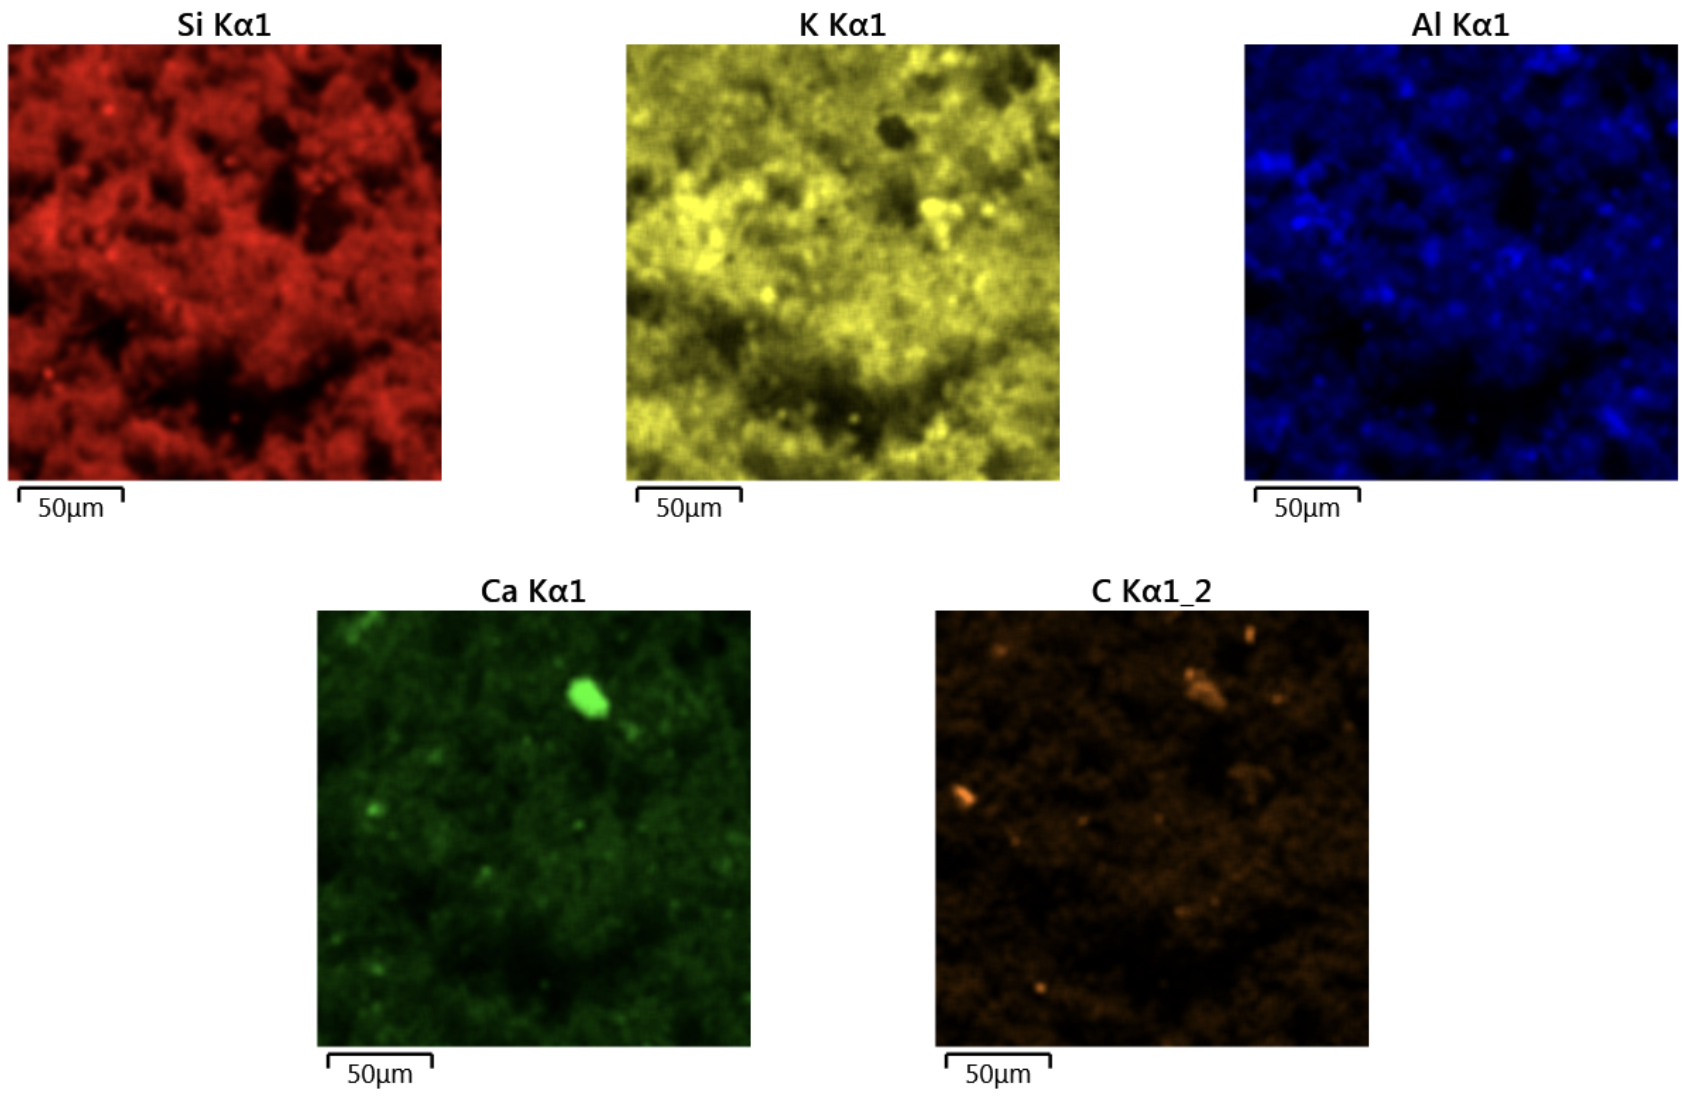
\includegraphics[height=6cm]{Cap4/images/3-0-60C-3d-Spot 3 - map.png}
    }
    \caption{EDS analysis of Spot 3, Si/Al = 3.0, cured for 3 days at 60°C at 1000× magnification.}
    \label{fig:eds_spot3_3-0}
\end{figure}

\begin{figure}[H]
    \centering
    \subfloat[EDS layered image]{
        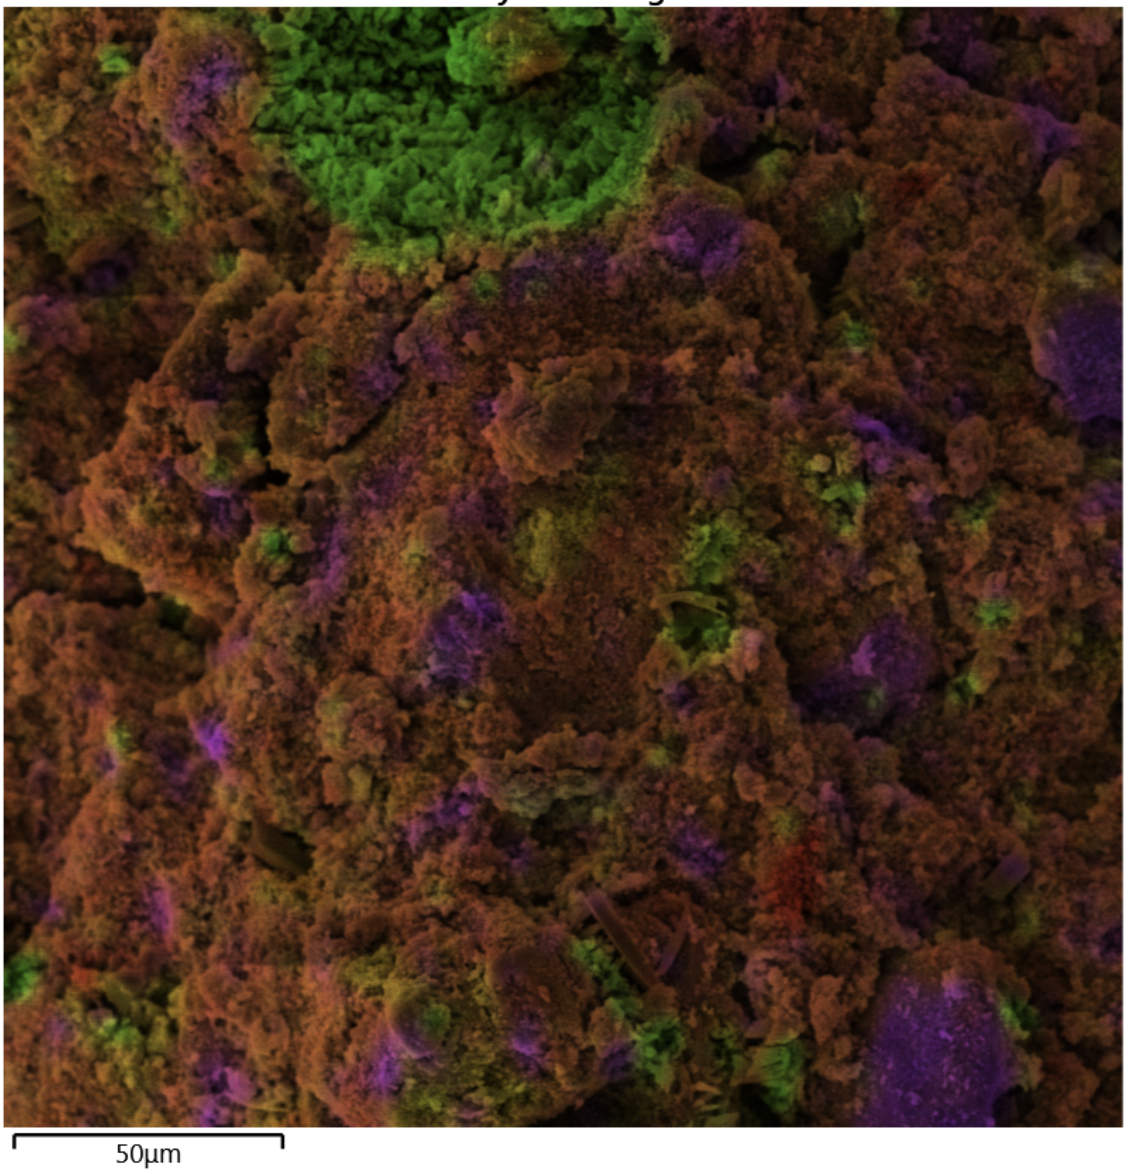
\includegraphics[height=6cm]{Cap4/images/5-0-60C-3d-Spot 1 - layered.png}
    }
    \hfill
    \subfloat[EDS map]{
        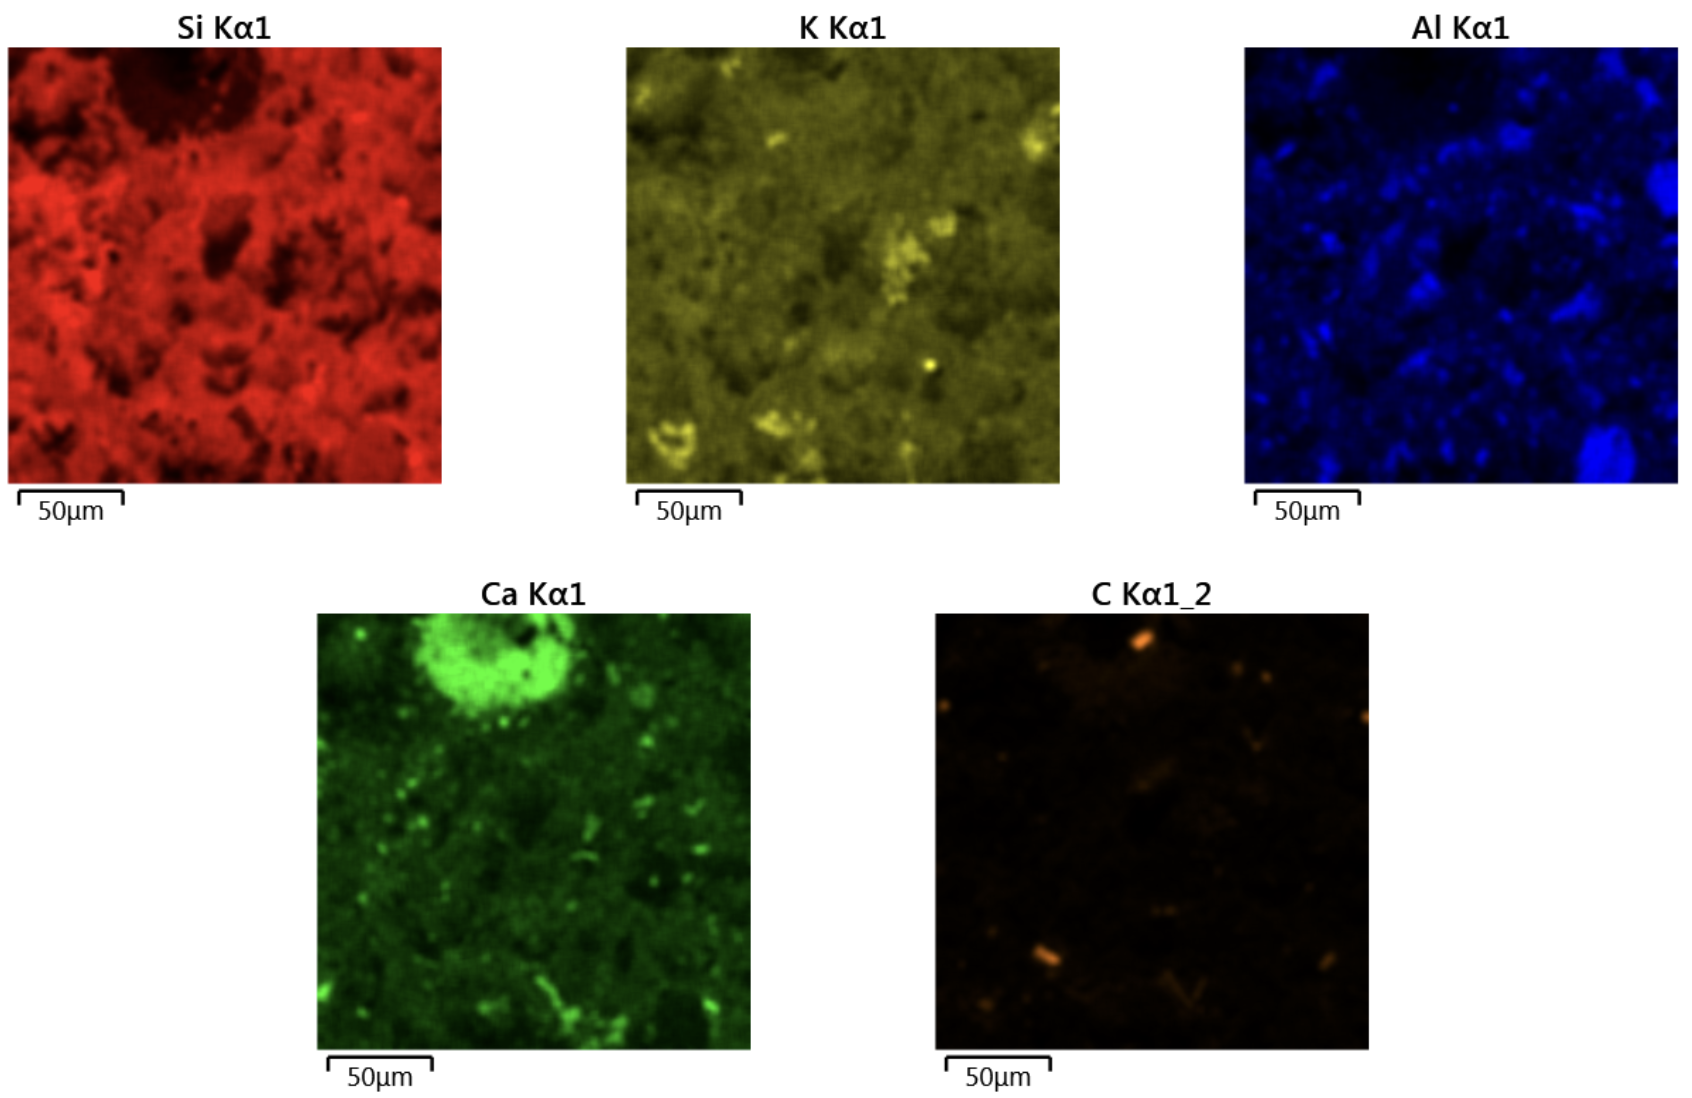
\includegraphics[height=6cm]{Cap4/images/5-0-60C-3d-Spot 1 - map.png}
    }
    \caption{EDS analysis of Spot 1, Si/Al = 5.0, cured for 3 days at 60°C at 1000× magnification.}
    \label{fig:eds_spot1_5-0}
\end{figure}

The spectrum results are summarized in Table \ref{tab:eds_spectrum} and it can be noted that the K/Ca ratio was approximately constant and equals to 2, as expected from the mix design.
However, the Si/Al ratio from EDS was slightly higher than the intended mix design values.
It can be speculated that this is due to a stronger tendency of Si to stays in solution rather than being incorporated into the gel structure and precipitate during geopolymerization at high pH environment \cite{chen2024synthesis}.
\textcolor{red}{Am I missing something?}

\begin{table}[H]
    \centering
    \caption{EDS spectrum of pastes after 3 days of curing at 60$\degree$C.}
    \label{tab:eds_spectrum}
    \begin{tabular}{l c c c c c c c c}
        \hline
        \multicolumn{1}{c}{Sample} & \multicolumn{4}{c}{At(\%)} & \multicolumn{4}{c}{Wt(\%)} \\
        \cline{2-9}
        & Si & Al & K & Ca & Si & Al & K & Ca \\
        \hline
        0.9\textunderscore 60C\textunderscore 3d\textunderscore Spot5 & 26.4 & 27.1 & 30.4 & 16.0 & 22.4 & 22.1 & 36.0 & 19.5 \\
        3.0\textunderscore 60C\textunderscore 3d\textunderscore Spot3 & 54.2 & 13.5 & 21.5 & 10.8 & 48.2 & 11.5 & 26.6 & 13.7 \\
        5.0\textunderscore 60C\textunderscore 3d\textunderscore Spot1 & 59.5 & 9.2 & 19.6 & 11.6 & 53.0 & 7.9 & 24.2 & 14.9 \\
        \hline
    \end{tabular}
\end{table}

Additional EDS spectral data for all analyzed spots can be found in Appendix \ref{appendix:eds_spectra}.




\subsection{X-Ray Diffraction}

X-ray diffraction patterns (3-day curing) of the pastes at different Si/Al ratios showed a persistent amorphous hump in all compositions, indicating the presence of aluminosilicate gel (N-A-S-H).
The hump position and shape were increasingly similar to the silica fume precursor at high Si/Al, consistent with the SEM observation, as it it shifted to the left as silica content increases. 

In agreement with other studies, the geopolymerization process—which is responsible for the strength—is indicated by the presence of the broad hump among $2\theta = 20 \approx 35\degree$.
process shifted the location of the amorphous hump to lower angles as the silica proportion increases \cite{arellano2014geopolymer,lee2017strength, wan2017geopolymerization}.

The patterns of the pastes show sharp peaks of crystalline phases of solid precursors, this indicates that the they were not involved in the geopolymerization process \cite{Geraldo2020}, but were rather present as inactive fillers, as noted by \cite{ruiz2012alkaline}.
The crystalline phases identified in the XRD patterns are presented in Table \ref{tab:xrd_phases_pastes}, showing the semi-quantitative phase composition at 3 days for different Si/Al ratios.

\begin{table}[H]
    \centering
    \caption{Semi-quantitative crystalline phases at 3 days for different Si/Al ratios (XRD).}
    \label{tab:xrd_phases_pastes}
    \begin{tabular}{lrrrrr}
        \hline
        \multicolumn{1}{c}{Phase (\%)} &
        \multicolumn{5}{c}{Si/Al}\\
        \cline{2-6}
        & 0.9 & 2.0 & 3.0 & 4.0 & 5.0 \\
        \hline
        Calcite (CaCO$_3$) & 77 & 56 & 43 & 52 & 79 \\
        Butschliite (K$_2$Ca(CO$_3$)$_2$) & 18 & 29 & 0 & 0 & 0 \\
        Aragonite (CaCO$_3$) & 0 & 0 & 41 & 24 & 0 \\
        Quartz (SiO$_2$) & 6 & 14 & 16 & 17 & 21 \\
        Stishovite (SiO$_2$) & 0 & 0 & 0 & 7 & 0 \\
        \hline
    \end{tabular}
\end{table}

Figure \ref{fig:xrd_pastes} exhibits that at lower Si/Al ratios, the peaks - specially from calcite - are more intense, indicating a higher presence of these crystalline phases from unreacted materials.

% Taken together, the XRD results corroborate the SEM/EDS findings: (i) all mixes formed an amorphous aluminosilicate gel, consistent with low-calcium N-A-S-H-type networks; (ii) Si/Al = 3.0 displayed the microstructurally densest matrix and, correspondingly, lower reliance on alkali-salt precipitation products; (iii) high Si/Al (4-5) retained unreacted silica, evidenced by the hump shape similarity to SA and the SiO₂ fraction; and (iv) low Si/Al (0.9) promoted alkali/carbonate crystallization (including butschliite) consistent with excess free alkali and early carbonation.

\begin{figure}[H]
    \centering
    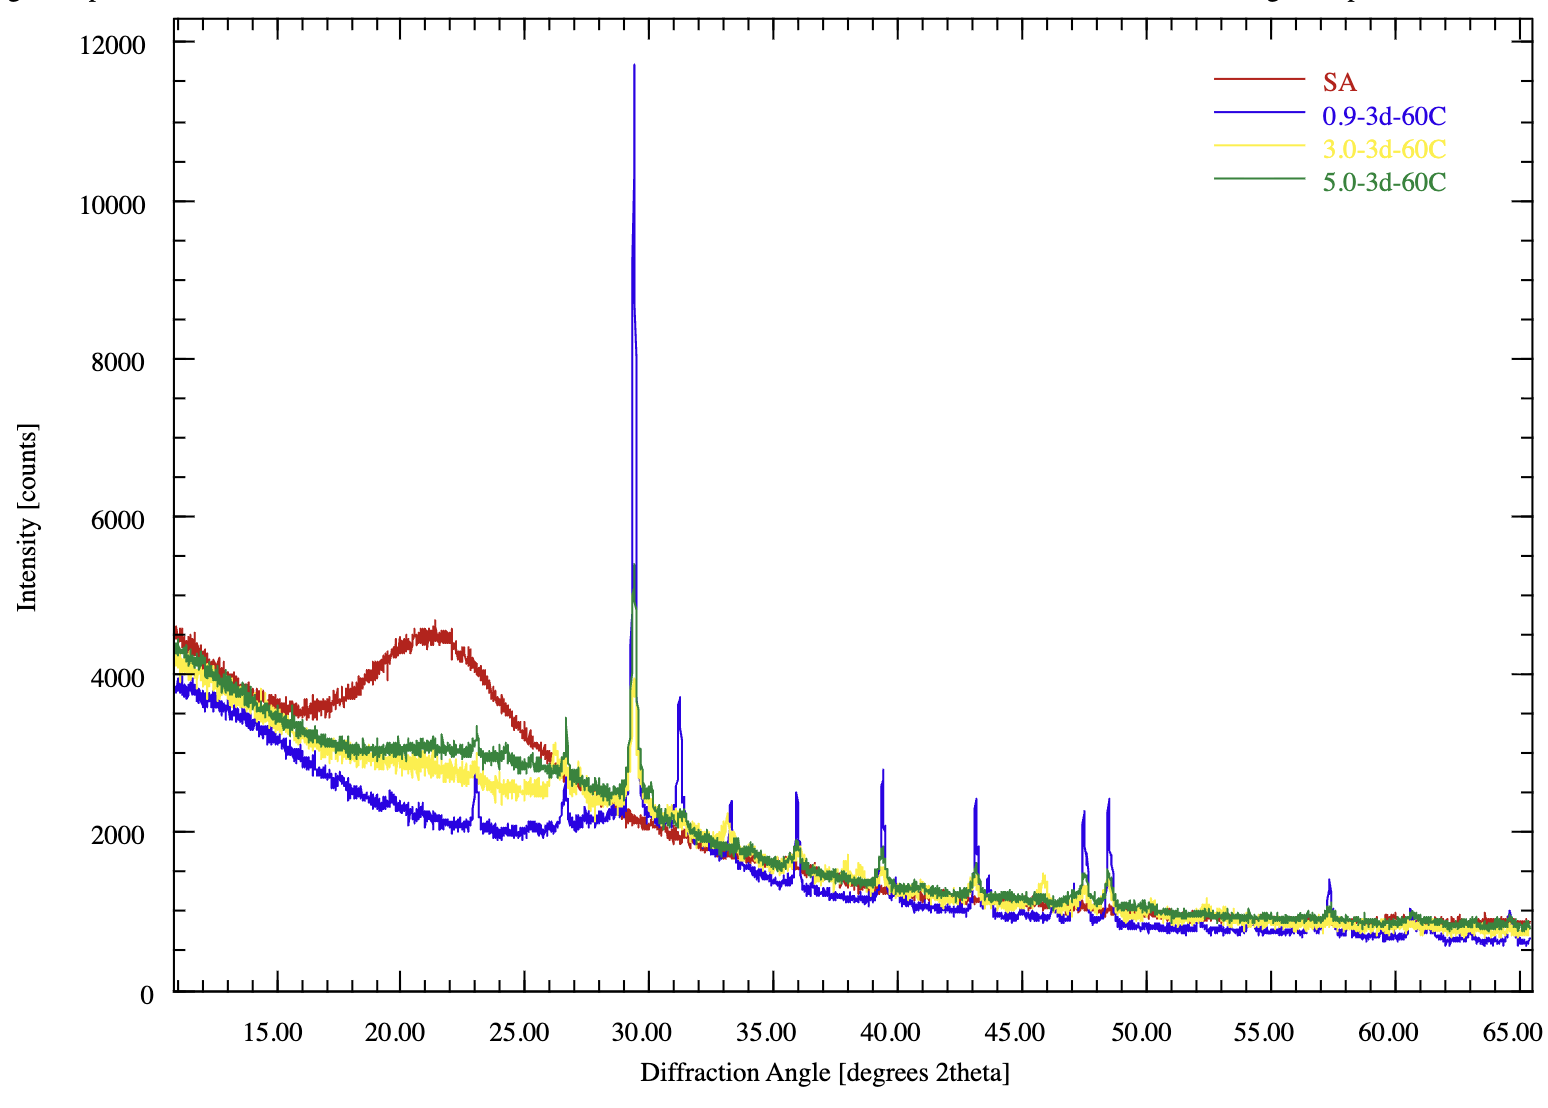
\includegraphics[width=0.8\textwidth]{Cap4/images/xrd_pastes.png}
    \caption{XRD patterns of pastes at different Si/Al ratios after 3 days of curing.}
    \label{fig:xrd_pastes}
\end{figure}

\textcolor{red}{Find a better way to present this graph, shifting vertically different rations and labeling the peaks.}

\subsection{Fourier Transform Infrared Spectroscopy}

FTIR spectra were collected for all pastes after 1 and 3 days of curing to analyze the chemical bonding and structural changes associated with geopolymerization at different Si/Al ratios.
There was no significant variation in the spectra from 1 to 3 days of curing, so only the spectra after 3 days are represented in Figure \ref{fig:ftir_pastes}.
The spectra of solid precursors are exhibited in Appendix \ref{appendix:ftir_spectra}.

\begin{figure}[H]
    \centering
    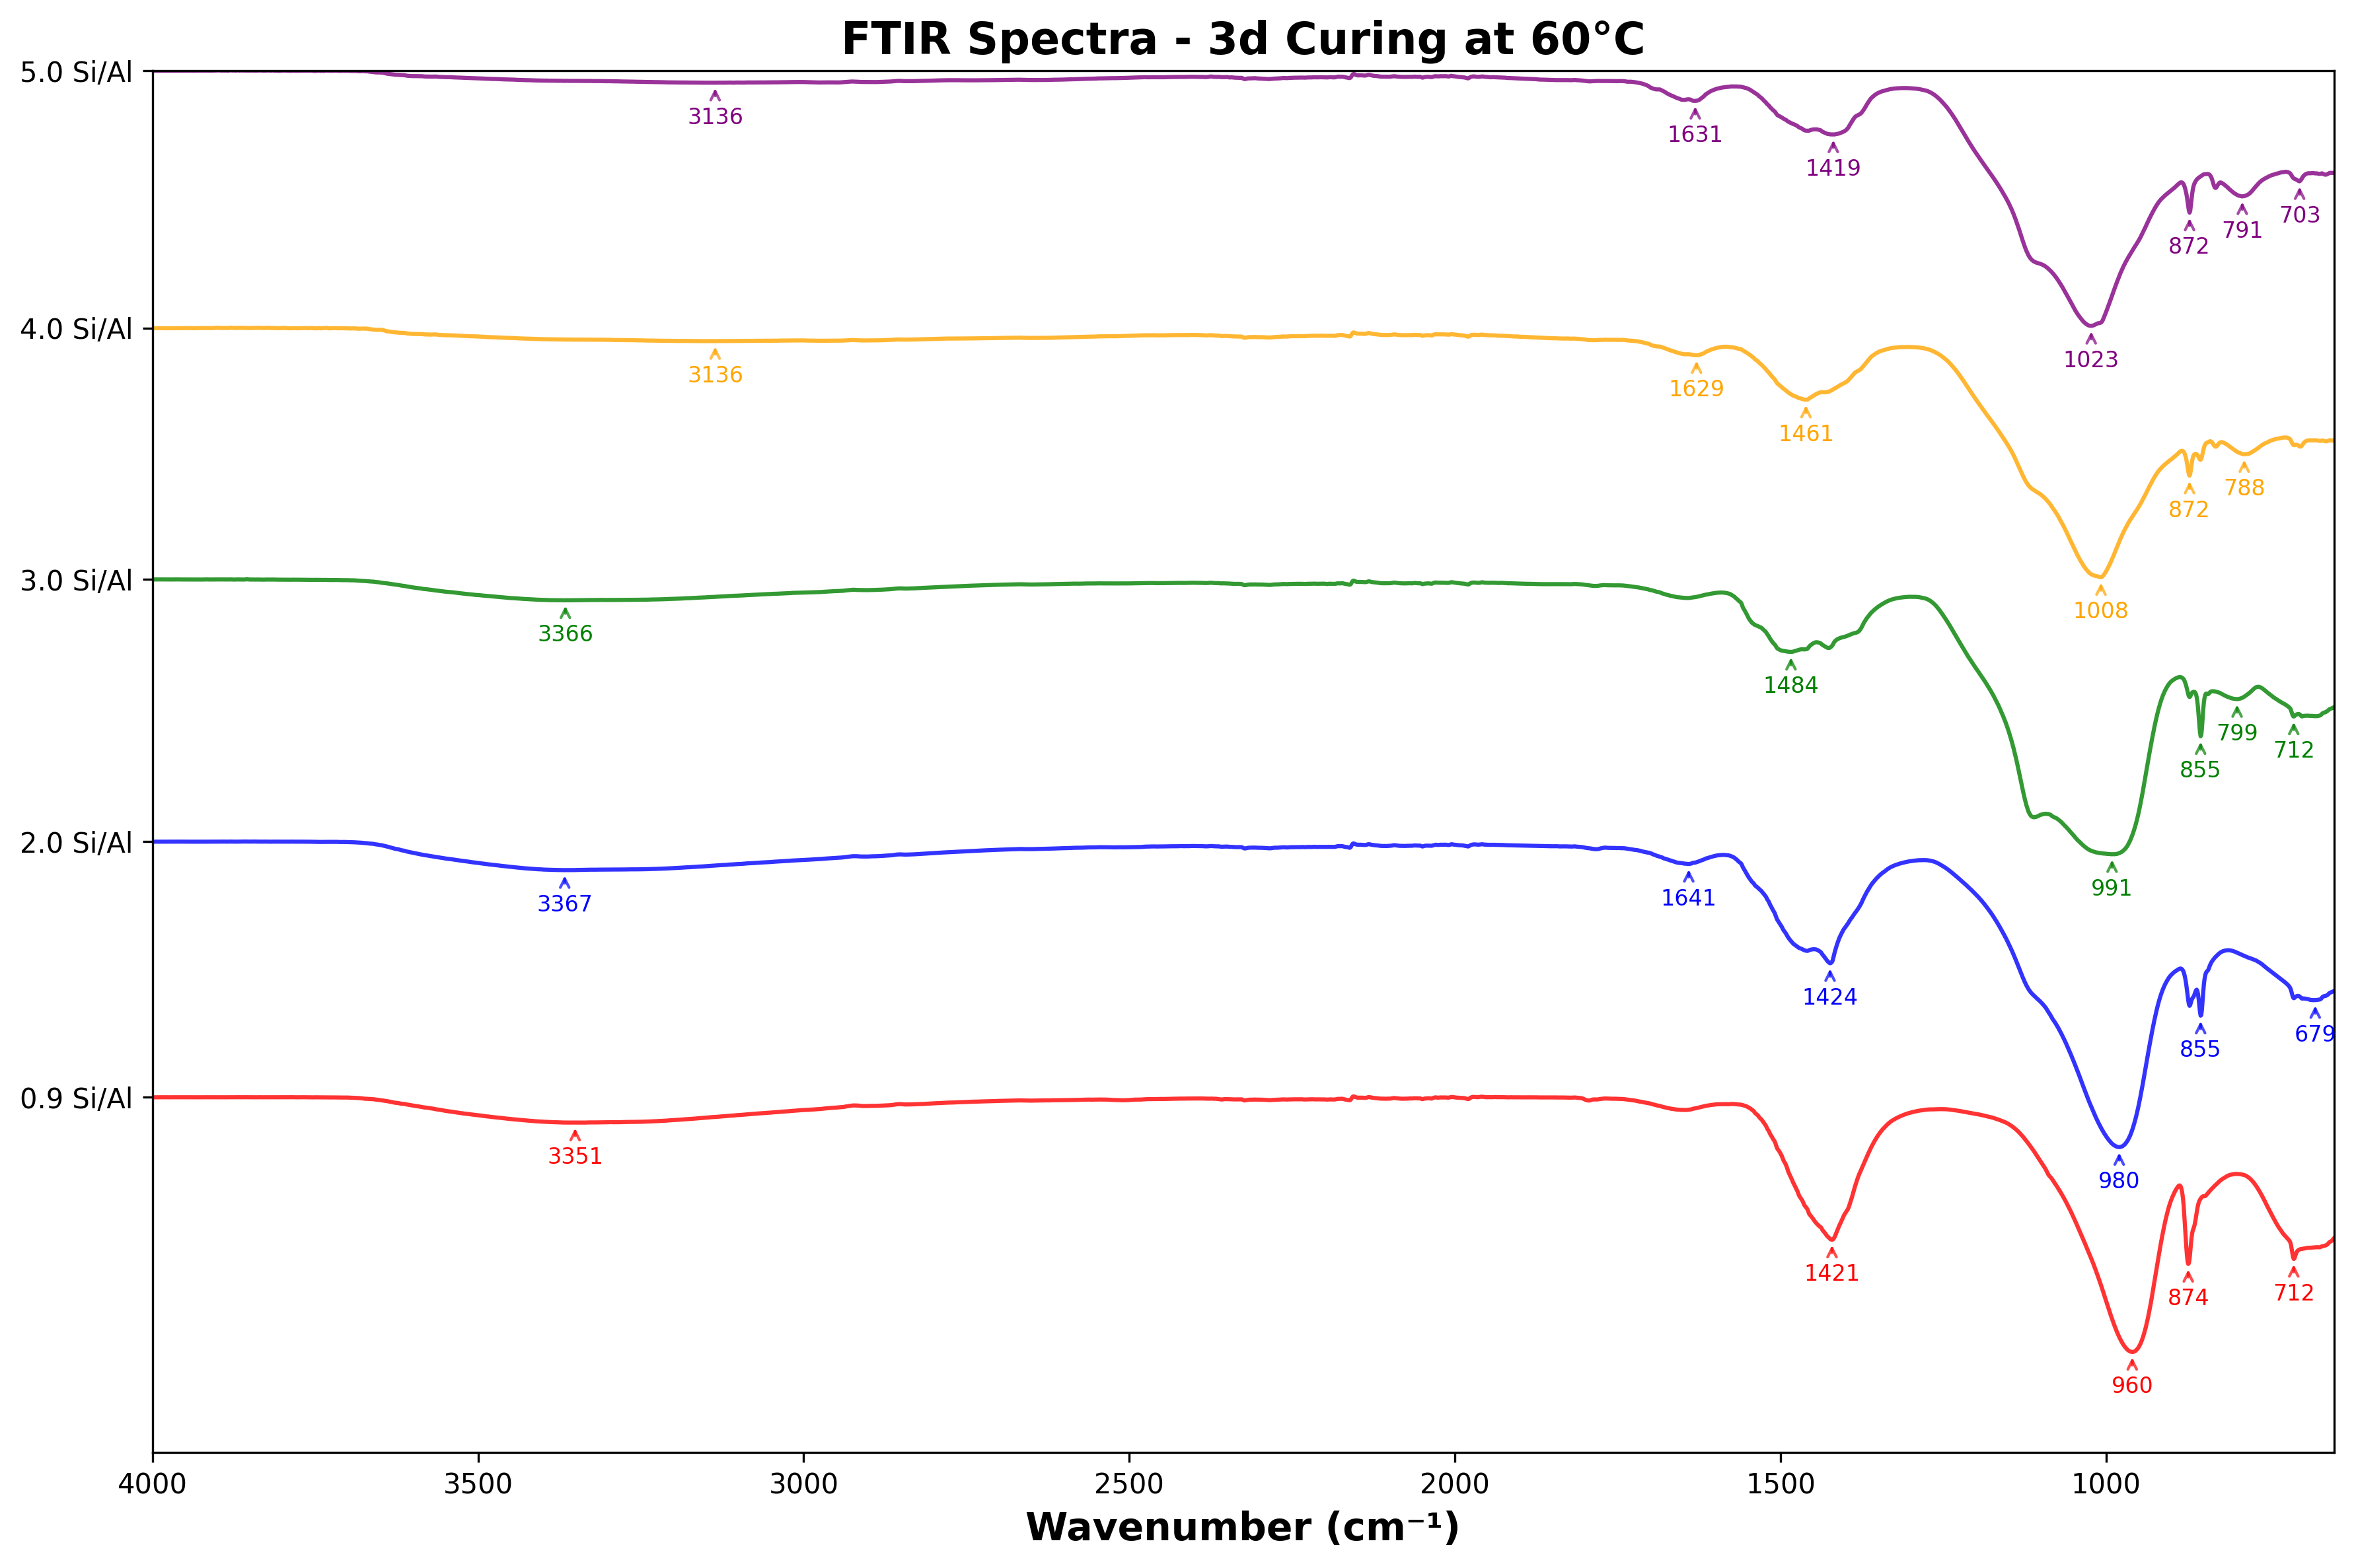
\includegraphics[width=0.8\textwidth]{Cap4/images/ftir_comparison_3d_curing.png}
    \caption{FTIR spectra of pastes at different Si/Al ratios after 3 days of curing.}
    \label{fig:ftir_pastes}
\end{figure}

The key to interpreting these spectra lies in the fingerprint region (400-1200 cm\textsuperscript{-1}), which reflects the formation of the polymeric network, and the hydroxyl/carbonate regions (1300-3700 cm\textsuperscript{-1}), which indicate water and carbonation.
The Table \ref{tab:ftir_assignments} summarizes the main FTIR peaks observed in the pastes and their assignments.

At lower Si/Al ratios, the reaction leads to a network with a higher density of Si-O-Al bonds, while the increasing Si content promotes the formation of Si-O-Si linkages, resulting in a more siliceous gel structure, shifting the main peak of Figure \ref{fig:ftir_pastes} towards higher wavenumbers, from 960 cm\textsuperscript{-1} (Si/Al = 0.9) to 1023 cm\textsuperscript{-1} (Si/Al = 5.0).
This means that the gel structure progressively replaces AlO\textsubscript{4}\textsuperscript{-} tetrahedra with SiO\textsubscript{4}\textsuperscript{-}, suggesting a higher degree of polymerization, denser and stronger molecular network \cite{pachecotorgal2014handbook}.

\begin{landscape}
    \begin{table}[p]
    \centering
    \caption{Assignment of FTIR absorption bands observed in pastes after 3 days of curing at 60$\degree$C, where T = Si or Al.}
    \vspace{0.5cm}
    {\small % Reduce font size for the table
    \renewcommand{\arraystretch}{1.2} % Increase row spacing
    \begin{tabular}{p{2.5cm} p{2.5cm} p{3cm} p{8cm} p{3cm}}
        \hline
        Wavenumber Range (cm$^{-1}$) & Observed Peaks & Vibration Mode & Chemical Significance & Reference \\
        \hline
        % 3641 & 3641 (Ca(OH)$_2$ precursor) & O-H stretching & Sharp band characteristic of crystalline portlandite (Ca(OH)$_2$). & \\
        3100-3450 & 3111, 3136, 3177, 3325, 3367 & O-H stretching & Represents weakly bonded or physically adsorbed water, and hydroxyl groups involved in hydrogen bonding within the gel structure. & \cite{Zhao2023}, \cite{provis2009geopolymers}, \cite{ma2022calcium}\\
        1620-1645 & 1629, 1631, 1632, 1641 & H-O-H bending & Vibration of interlayered or physically bound water molecules in the AAM matrix. & \cite{Zhao2023}, \cite{pachecotorgal2014handbook}\\
        1350-1500 & 1419, 1423, 1461, 1484 & C-O stretching & Characteristic of carbonates, indicating atmospheric carbonation (formation of CaCO$_3$ or K$_2$CO$_3$). & \cite{Zhao2023}, \cite{pachecotorgal2014handbook}, \cite{moraes2024scsa}\\
        950-1100 & 960, 1008, 1023 & Si-O-T asymmetric stretching & Primary diagnostic band of N-A-S-H gel formation. Shifted to lower frequencies when compared to precursors (SA: 1040, MK: 1051 cm$^{-1}$) indicates precursor dissolution and gel polymerization. & \cite{ma2022calcium}, \cite{Zhao2023}, \cite{provis2009geopolymers}\\
        780-880 & 787, 855, 872 & Si-O-Si symmetric stretching or C-O bending & Peaks around 780-800 cm$^{-1}$ relate to unreacted quartz. Bands in 850-880 cm$^{-1}$ are associated with carbonate bending vibrations. & \cite{moraes2024scsa}, \cite{pachecotorgal2014handbook}\\
        550-700 & 563, 679, 703, 712 & O-T-O or Al-O-T bending & Associated with bending vibrations in the tetrahedral network, specifically Al-O linkages in AlO$_4$ units or O-Si-O bending. & \cite{Zhao2023}, \cite{ma2022calcium} \\
        \hline
    \end{tabular}
    }
    \label{tab:ftir_assignments}
    \end{table}
\end{landscape}

\chapter{Conclusion}
Lorem ipsum dolor sit amet, consectetur adipiscing elit. Nullam venenatis augue id augue ultrices, et gravida magna vehicula. Cras volutpat suscipit iaculis. Praesent varius ac orci sed ultrices. Vivamus vestibulum molestie lorem. Maecenas id congue tortor. Aliquam erat volutpat. Nullam ornare tortor et nunc sagittis laoreet. Sed at turpis et quam facilisis elementum. Nullam ultrices elit ut accumsan ultricies. Nulla sit amet tellus lacus. Vestibulum ac lectus velit. Donec nunc odio, mattis nec orci sed, porta lobortis lectus.

Proin ultricies elit vitae mi efficitur eleifend. Nulla non lorem consectetur, placerat dui quis, feugiat urna. Quisque sed ligula massa. Donec finibus placerat orci, eget mollis justo rutrum a. Sed luctus feugiat congue. Phasellus libero felis, tempor quis rutrum pretium, porttitor ac nisi. Praesent euismod malesuada enim a rhoncus. Aliquam gravida fringilla aliquam. Proin nunc lorem, convallis fringilla eleifend et, tempus quis orci. Phasellus bibendum, tellus eu elementum posuere, odio lacus maximus eros, nec lobortis lectus nisi a turpis. Vivamus viverra felis et dolor viverra interdum. Nulla convallis nisi eu sapien egestas aliquet sit amet eget risus. Phasellus vel quam vel lacus commodo lacinia.

Donec ultrices ac nisi nec elementum. Aenean pellentesque pellentesque pulvinar. Ut aliquet nulla vitae porttitor hendrerit. Nullam venenatis nisl nec ipsum malesuada ultricies. Curabitur massa erat, auctor in ipsum non, semper ornare nunc. Donec non felis eget diam porta rhoncus. Mauris id lectus sed arcu iaculis dictum et vitae velit. Cras sit amet neque vel sapien interdum fermentum sit amet eu lorem. Fusce urna sem, pretium a facilisis id, aliquet at mi. Etiam elementum eget est et porttitor. Morbi ultricies lorem a arcu mattis, eget egestas ex ultrices. Pellentesque bibendum sed est ac imperdiet.

% REFERENCIAS BIBLIOGRAFICAS
\renewcommand\bibname{\itareferencesnamebabel} %renomear título do capítulo referências
\bibliography{References/references}

% Apendices
\appendix
\chapter{Mix Design Formulations} %optional
\section{A First Section for the Appendix}

The Linear Dilemma matrix $M$ and the inertial torque vector $b$, used in the simulation, are calculated according to the formulation below:
\begin{equation}
M=\left[ \begin{array}{ccc}
M_{11} & M_{12} & M_{13} \\
M_{21} & M_{22} & M_{23} \\
M_{31} & M_{32} & M_{33}
\end{array} \right]
\end{equation}

% \begin{figure}[h]
% \centering
% \includegraphics[height=5cm, width=5cm]{ApeA/pragas_ciclo_cupim}
% \caption{A figure that is in the appendix}\label{FD}
% \end{figure}


% Anexos
% \annex
% \chapter{First annex example} %optional
% \section{Annex A: Example of Annex}
\label{anexoA}


Example of a table.

\begin{table}[ht]
\caption{Example of a Table}
\label{minhatab}

\center
\begin{tabular}{cccc}
  % after \\: \hline or \cline{col1-col2} \cline{col3-col4} ...
  \hline
	Parameter & Unit & Simulation value & Experimental value   \\
	\hline
  Length, $\alpha$ & $m$ &  $8.23$  & $8.54$ \\
  Height, $\beta$ & $m$     &  $29.1$ & $28.3$\\
	Velocity, $v$ & $m/s$  &  $60.2$ & $67.3$\\
	\hline
\end{tabular}
\end{table}

% Example of a figure.

% \begin{figure}[ht]
% \centering
% \includegraphics[width=0.75\textwidth]{Cap2/spiderrobot}
% \caption{Cybernetic termite.}\label{fig:cupim}
% \end{figure}


Example of an equation

\begin{equation} \label{eq:lagr1}
\frac{d}{dt}(\frac{\partial L}{\partial \dot{q}})-\frac{\partial L}{\partial q}=\tau^{T}.
\end{equation}



% Glossario
%\itaglossary
%\printglossary

% Folha de Registro do Documento
% Valores dos campos do formulario
\FRDitadata{26 de maio de 2025}
\FRDitadocnro{DCTA/ITA/DM-018/2025} %(o número de registro você solicita a biblioteca)
\FRDitaorgaointerno{Aeronautics Institute of Technology -- ITA}
%Exemplo no caso de pós-graduação: Instituto Tecnol{\'o}gico de Aeron{\'a}utica -- ITA
\FRDitapalavrasautor{AAM; Geopolymer; One-part}
\FRDitapalavrasresult{AAM; Geopolymer; One-part}
%Exemplo no caso de graduação (TG):
%\FRDitapalavraapresentacao{Trabalho de Graduação, ITA, São José dos Campos, 2015. \NumPenultimaPagina\ páginas.}
%Exemplo no caso de pós-graduação (msc, dsc):
\FRDitapalavraapresentacao{ITA, São José dos Campos. Undergraduate Course. Undergraduate Program in Civil-Aeronautical Engineering. Department of Structures and Buildings. Advisor: Prof.~Dr. João Cláudio Bassan de Moraes. Co-advisor: Pamela Rodrigues Passos Severino. Defense on 05/26/2025. Published on 05/26/2025.}
\FRDitaresumo{Na busca por alternativas mais sustentáveis ao cimento Portland, os cimentos ativados alcalinamente têm sido amplamente estudados.
Inicialmente, a maioria dos processos de mistura ocorre em duas etapas, que sacrificam a eficiência produtiva em função das melhores proriedades mecânicas.
Com o objetivo  aumentar a escalabilidade do processo, o desenvolvimento de sistemas monocomponentes trouxe uma tecnologia mais acessível e prática para a indústria.
Ainda assim, os estudos atuais se concentram em precursores ricos em
cálcio, enquanto o uso de fontes alcalinas tradicionais apresenta desafios relacionados à segurança e ao custo.
Este trabalho propõe o desenvolvimento de um cimento ativado alcalinamente monocomponente utilizando precursores sólidos de baixo teor de cálcio, como sílica ativa e metacaulim, e fontes alcalinas mais seguras e acessíveis, como carbonato de potássio e hidróxido de cálcio, garantindo resistência mecânica adequada e maior viabilidade para aplicação na construção civil.}
%  Primeiro Parametro: Nacional ou Internacional -- N/I
%  Segundo parametro: Ostensivo, Reservado, Confidencial ou Secreto -- O/R/C/S
\FRDitaOpcoes{N}{O}
% Cria o formulario
\itaFRD

\end{document}
% Fim do Documento. O massacre acabou!!! :-)
